
\chapter{Function Spaces}
\label{ch:function:space}

\section{Distributions}

Distributions are the bras (dual vectors) of function space. They are almost functions, but they are waiting to be integrated. They are the analog of the definition of dual vectors through the inner product
\begin{align}
    \row{v} \defeq \la \vec{v}, \Vtextvisiblespace[1em]{}\, \ra \ .
\end{align}
In a function space the inner product is some kind of integral. A distribution is an additional weighting factor.\sidenote{You may want to compare this to related ideas: kernels and convolutions.}







\section{Functions as Vectors}

Functions are vectors in a vector space that we call \textbf{function space}\index{function space}. I am pretty sure that mathematicians do not call it that, but we use this terminology anyway. That functions can form a vector space should be \emph{obviously} true after our examination of the Fourier series and Fourier transform. Consider two polynomial functions $f$ and $g$. Maybe
\begin{align}
  f(x) &= x^3  
  &
  g(x) &= x + 2 \ ,
\end{align}
though the precise forms do not matter. Clearly you can take a linear combination of the two and the result is also a polynomial function:
\begin{align}
  \alpha f(x) + \beta g(x) = \alpha x^3 + \beta x + 2\beta \ .
\end{align}
This is a totally valid function that we could call $(\alpha f + \beta g)(x)$. 

In this example, it does not matter at all that the functions/vectors are themselves linear maps from $\RR \to \RR$.\sidenote{This should sound familiar. The dual vector space $V^*$ of row vectors are simultaneously a ``vector space in itself'' and a space of functions from $V\to \RR$.} All that matters is that the function/vectors have components that add linearly when we take linear combinations. Of course, the components are components \emph{with respect to a basis}. Let us restrict to the class of polynomials up to degree $N$, so these are functions of the form
\begin{align}
    f(x) = a^0 + a^1 x + a^2 x^2 + \cdots + a^N x^N \ .
\end{align}
Okay, the indices are a little annoying. The components $a^N$ have an upper index because they are components of a vector. The monomials $x^n$ are actual powers of the variable $x$. Evidently, these $(N+1)$ monomials are our basis for polynomial space.\sidenote{The vector space is $(N+1)$-dimensional because we include the constant, $x^0$.} 
\begin{align}
    \ket{e_n} &= x^n
    &
    n \in \{0, 1, 2, \cdots, N\} \ .
    \label{eq:polynomial:basis}
\end{align}
Note that we have not said anything about whether this basis is orthonormal or not---we have not yet defined a metric for this polynomial space. 

It is clear that the an $N$-component column vector encodes the information of a function:
\begin{align}
    \ket{f} &= 
    \begin{pmatrix}
        a^0 \\ a^1 \\ a^2 \\ \vdots \\ a^N
    \end{pmatrix} 
    &
\ket{f} &= 
    \begin{pmatrix}
        b^0 \\ b^1 \\ b^2 \\ \vdots \\ b^N
    \end{pmatrix} 
    \ .
\end{align}
Further, one may take linear combinations of these columns to encode linear combinations of functions:
\begin{align}
    \ket{\alpha f + \beta g}
    &= 
    \begin{pmatrix}
        \alpha a^0 + \beta b^0 \\ \alpha a^1 + \beta b^1 
        \\ \alpha a^2 + \beta b^2 \\ \vdots \\ 
        \alpha a^N + \beta b^N
    \end{pmatrix}  \ .
\end{align}

We can take $N$ to be as large as we want. In fact, if we go to $N\to \infty$, we can reproduce any function that admits a Taylor expansion. As physicists we will take this limit cavalierly. There are a few subtleties that show up that we will point out, but we will not let ourselves get bogged down in mathematical detail. Welcome to the world of infinite-dimensional vector spaces. We call these spaces \textbf{Hilbert spaces}.

A judicious choice of basis for function space can make our lives much easier. This is a central theme of this course and justifies the beastiary of special functions that you meet in graduate school. Let us ignore the subtleties of defining a function space for now---we get to this soon enough. The following example gives a taste of what it means to work with functions as vectors.


\begin{exercise}
%https://math.stackexchange.com/questions/942263/really-advanced-techniques-of-integration-definite-or-indefinite/943212

Here is a cute two-dimensional function space that gives us a shortcut to calculate a particular \emph{indefinite} integral.  Consider a two dimensional vector space spanned by the functions
\begin{align}
  \left|f_1\right\rangle
  &= f_1(x) = 
  e^{ax} \cos bx
  &
  \left|f_2\right\rangle
  &=
  f_2(x) = 
  e^{ax} \sin bx \ ,
\end{align}
where $a$ and $b$ are constants. Forget orthonormality or boundary conditions for this problem. The derivative $d/dx$ is a linear operator that acts on this space. Write down the derivative as a $2\times 2$ matrix in the above basis, $D$.

Invert $D$ in the usual way that you learned to invert $2\times 2$ matrices during your childhood\footnote{Stuck? Here's a life pro tip: \url{http://bfy.tw/KG2Z}}. Call this matrix $D^{-1}$. 

Now stop and think: the inverse of a derivative is an indefinite integral\footnote{Ignore the constant term.}. Thus acting with $D^{-1}$ on the vector $|f_1\rangle$ should be understood as an integral of $f_1(x)$. Show that, indeed,
\begin{align}
  D^{-1} |f_1\rangle = \int dx\, e^{ax} \cos bx \ .
\end{align}
Feel free to use \emph{Mathematica} to do the indefinite integral on the right-hand side. Pat yourself on the back if you can do it without a computer.
\end{exercise}


\section{Histogram Space}
\label{sec:histogramspace}

Here is a funny vector space that we call \emph{histogram space}. The basis vectors are:

\begin{center}
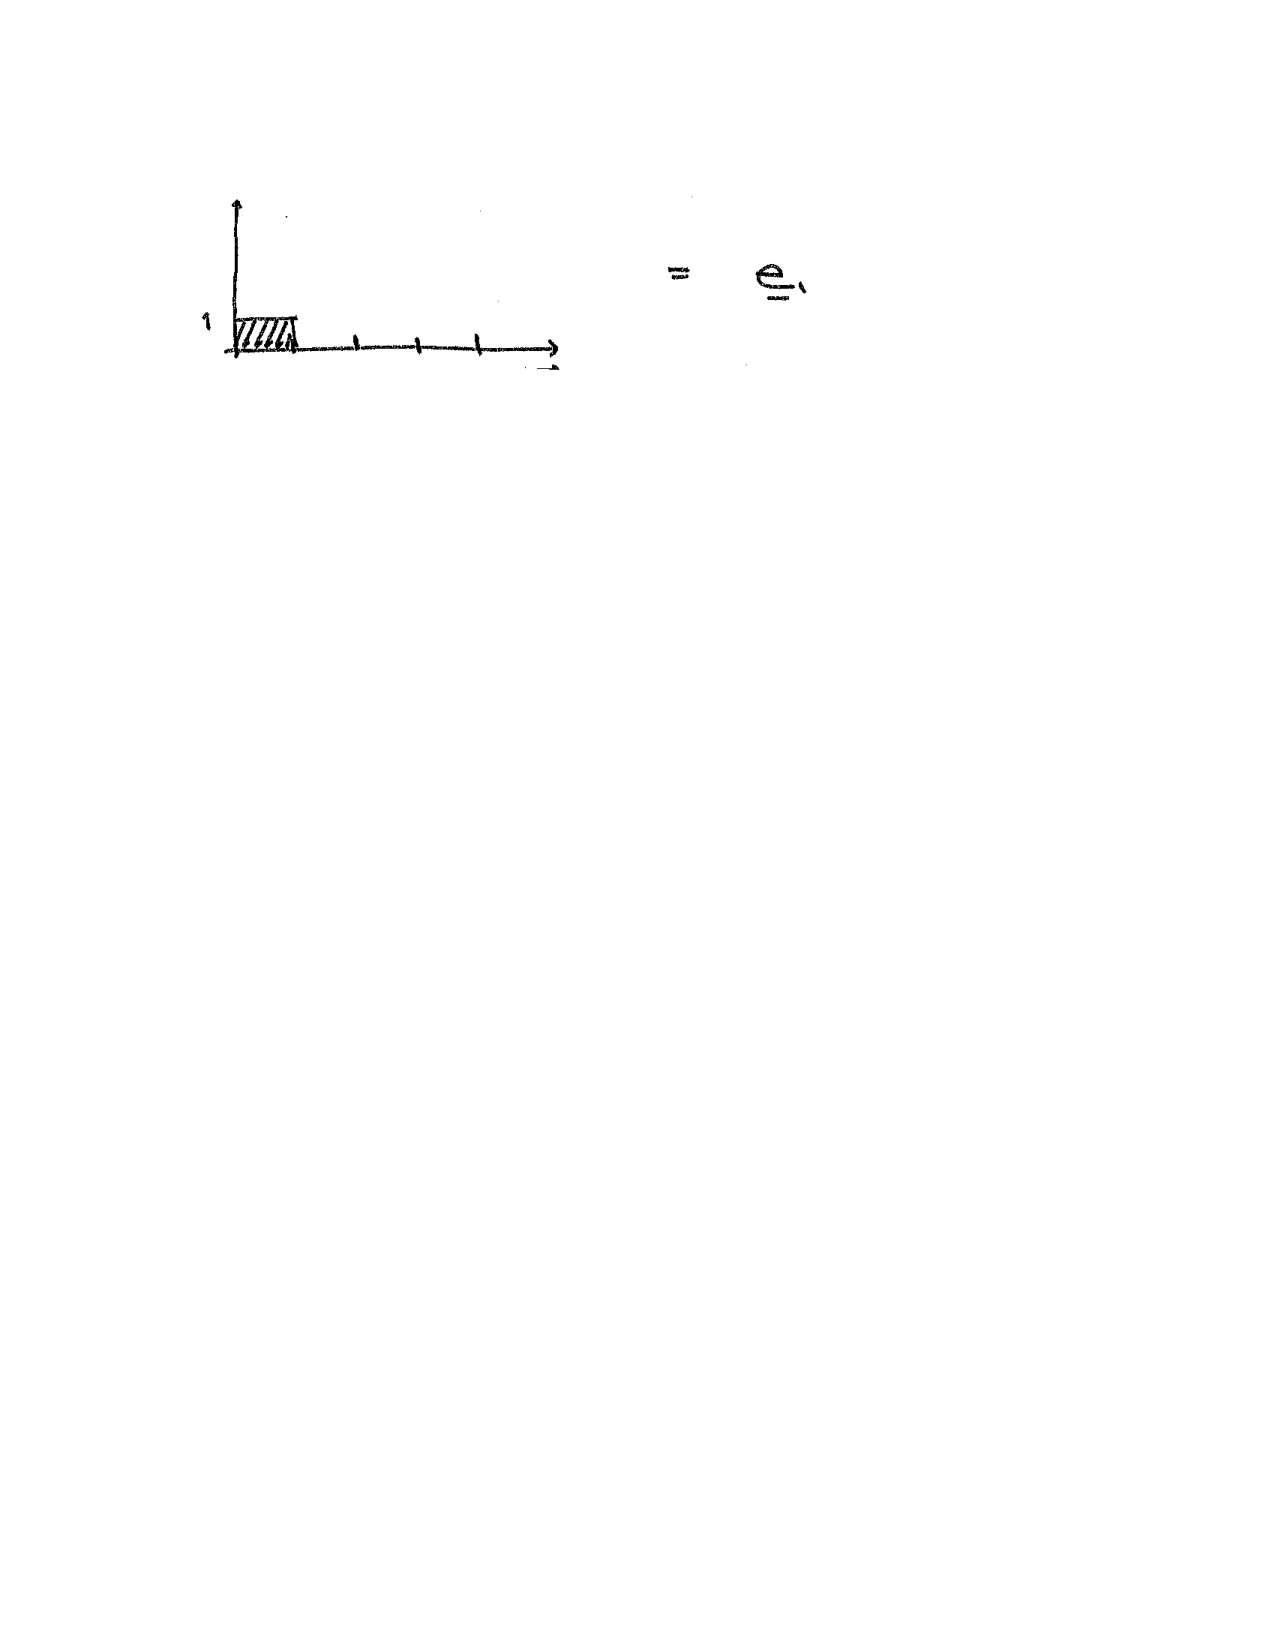
\includegraphics[width=.45\textwidth]{figures/lec02_e1.pdf}
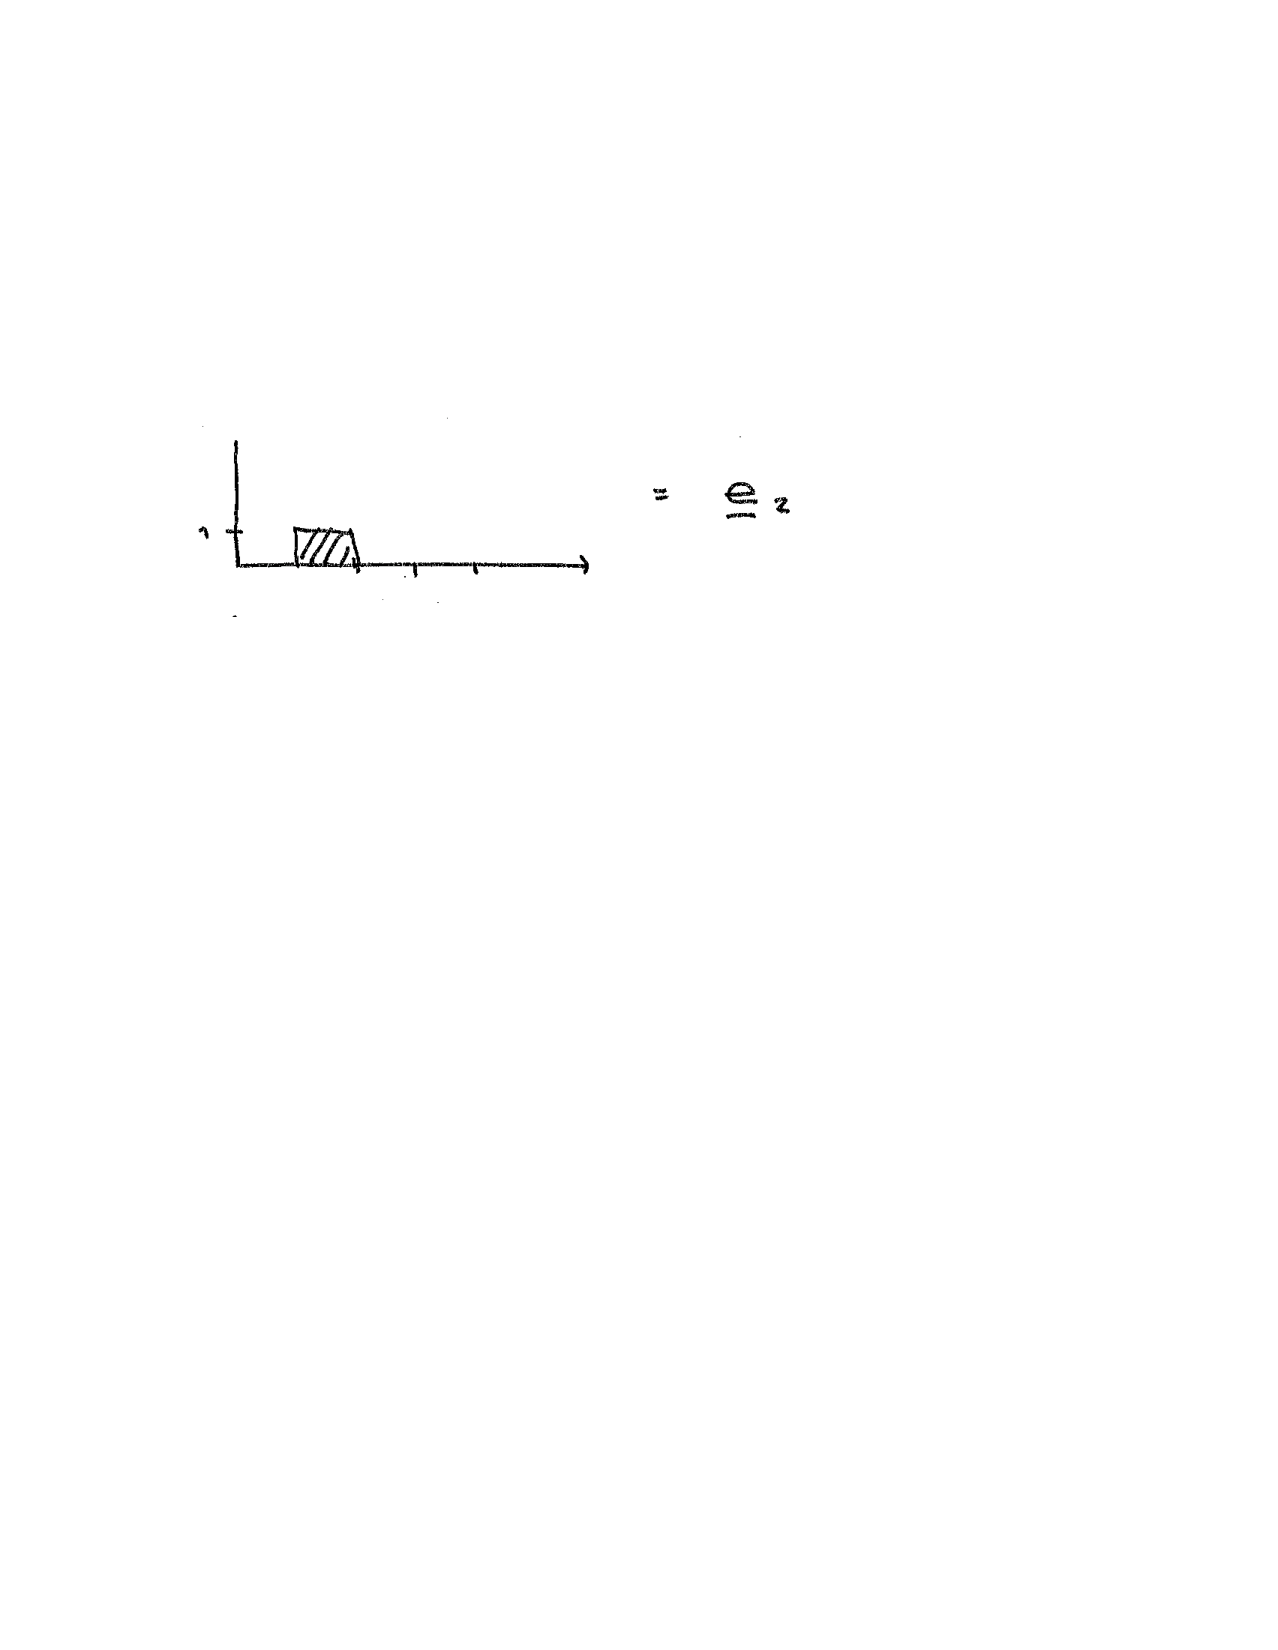
\includegraphics[width=.45\textwidth]{figures/lec02_e2.pdf}\\
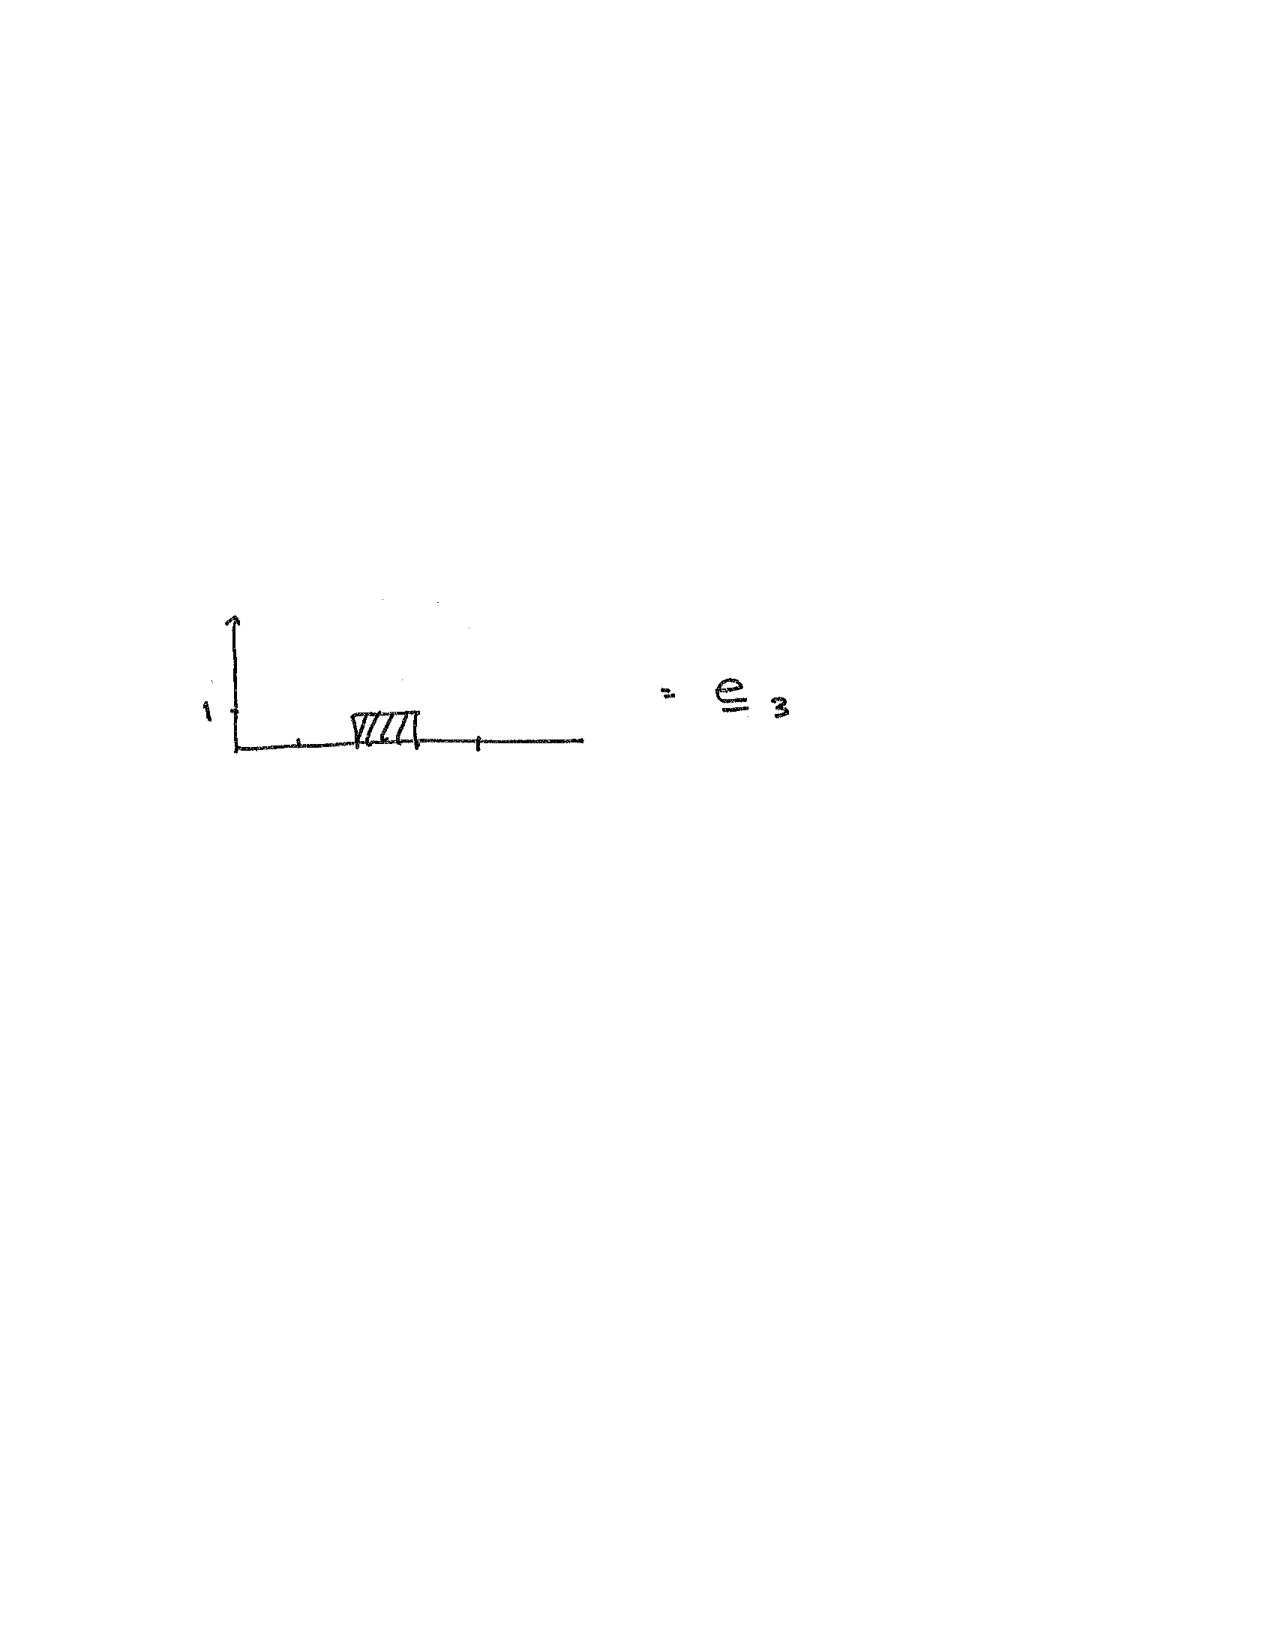
\includegraphics[width=.45\textwidth]{figures/lec02_e3.pdf}
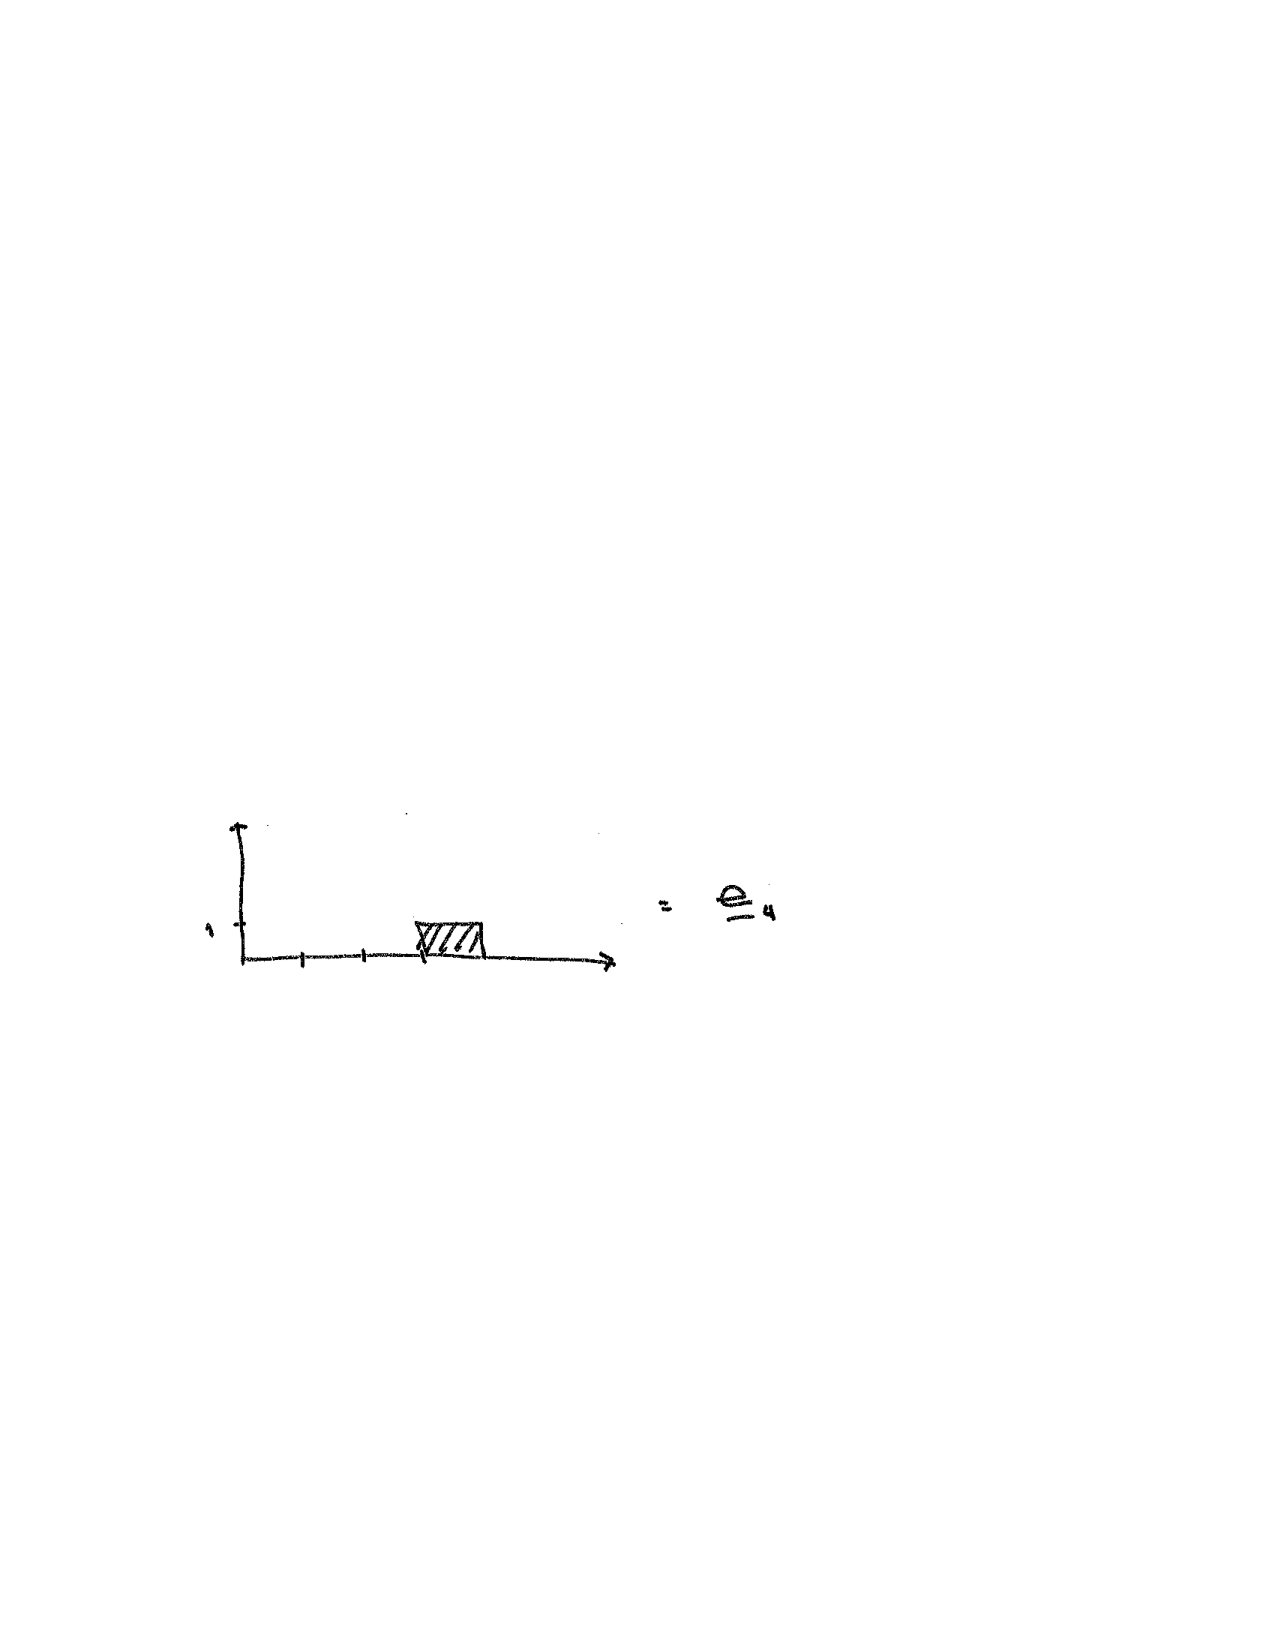
\includegraphics[width=.45\textwidth]{figures/lec02_e4.pdf}
\end{center}

\noindent This is a basis for a histogram over unit bins from $x=0$ to $x=4$. A vector in this space is, for example:

\begin{center}
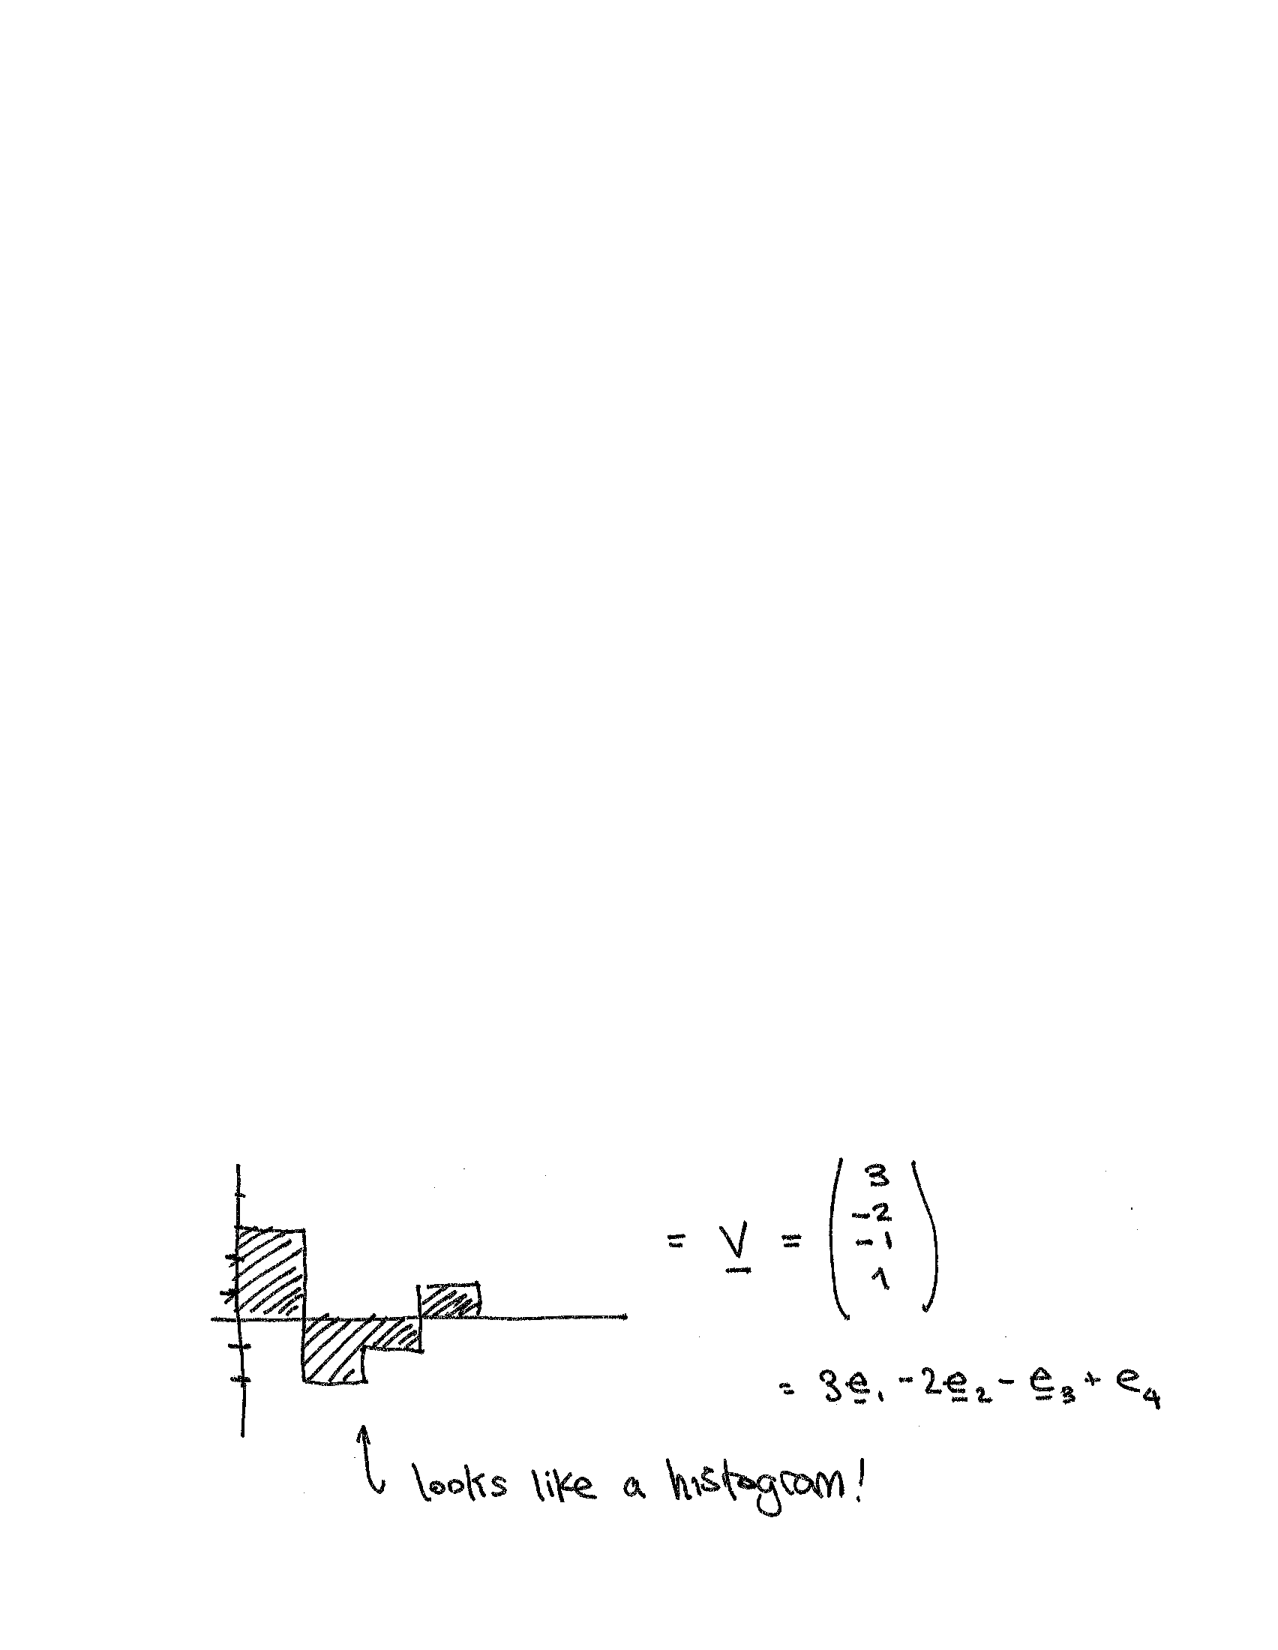
\includegraphics[width=.8\textwidth]{figures/lec02_hist.pdf}
\end{center}

\noindent We can perform a linear transformation $A$ on $\vec{v}$ which outputs another vector. Let us say it is this:
\begin{center}
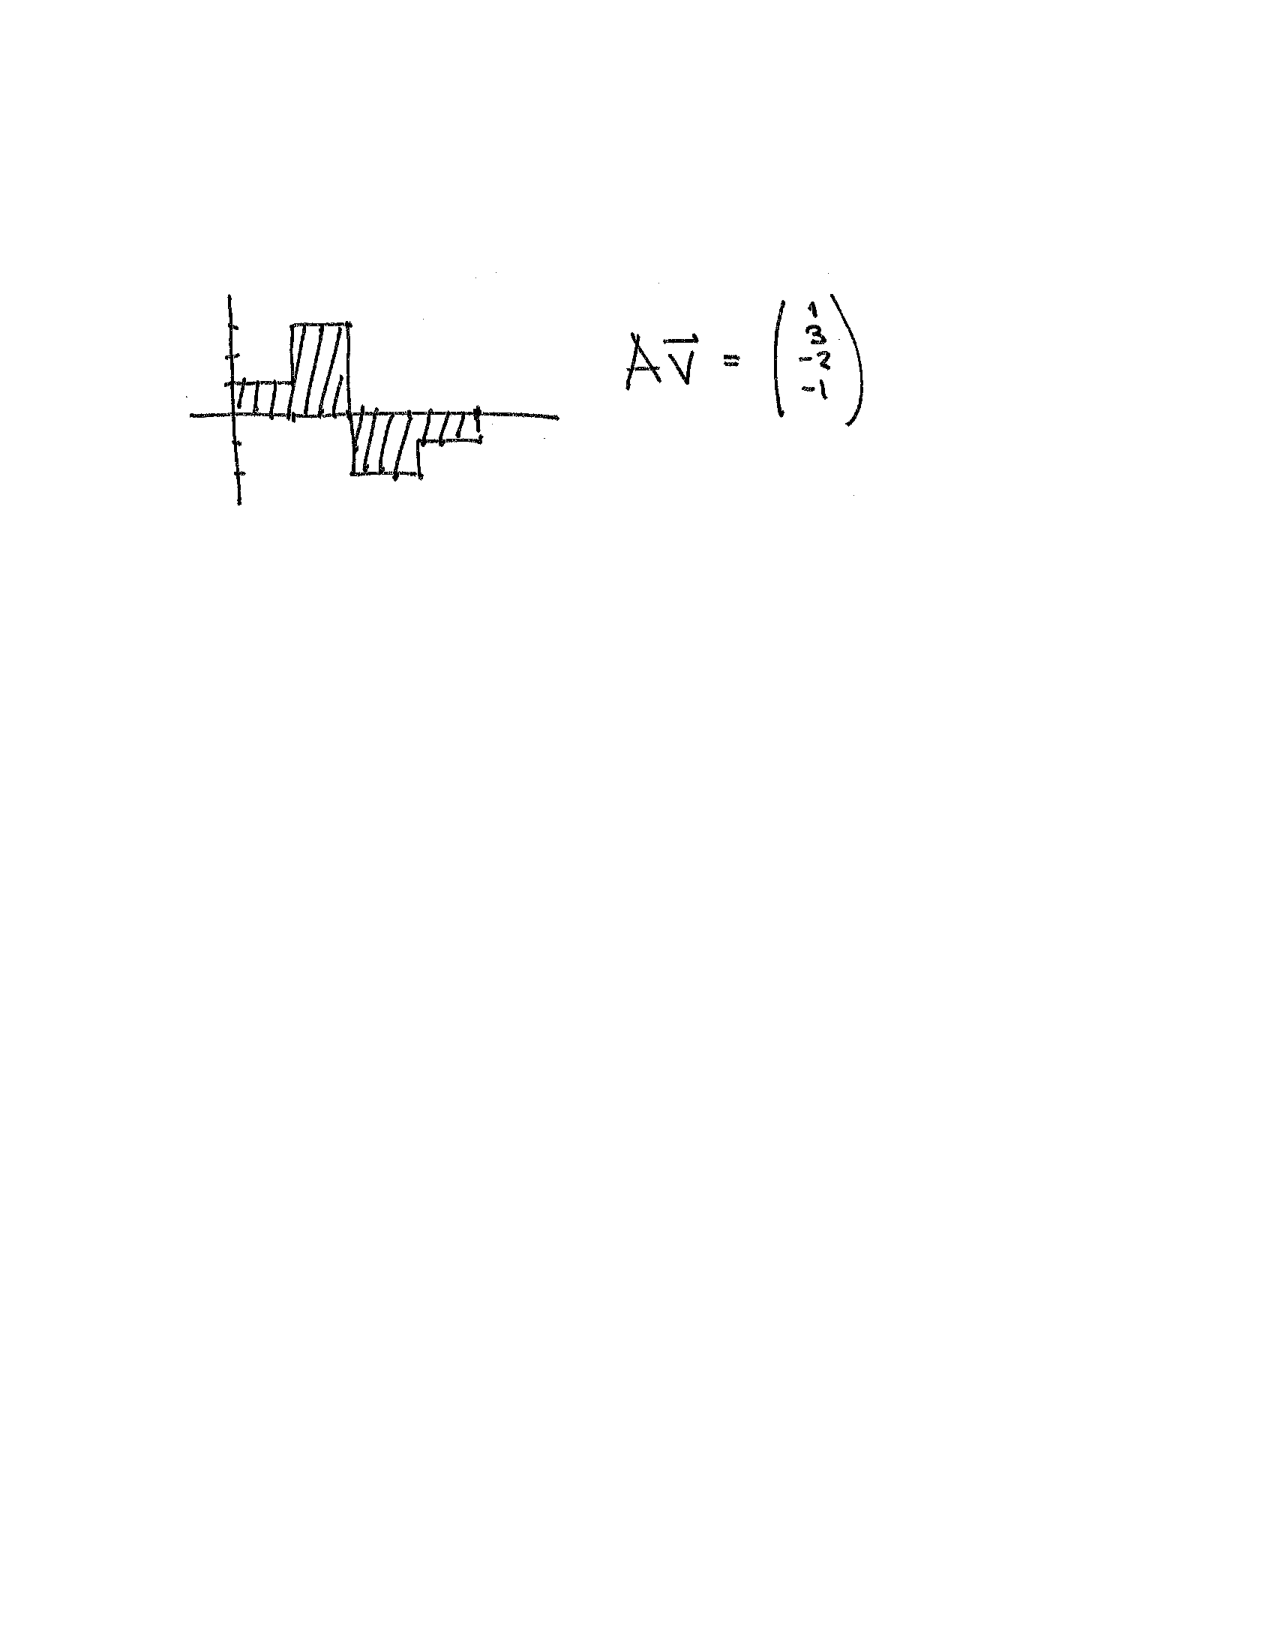
\includegraphics[width=.8\textwidth]{figures/lec02_hist2.pdf}
\end{center}

\begin{exercise}
From the image above, can you derive what $A$ is? 
\end{exercise}

\noindent The answer to the above exercise is \emph{no}. Please make sure you convince yourself why: there are many different transformations that convert to old histogram into the new histogram. The matrix $A$ is $4\times 4$ and thus has 16 entries that we need to define. The matrix equation $A\vec{v} = \vec{w}$ for known vectors $\vec{v}$ and $\vec{w}$ encodes only four equations.

The power of this admittedly strange vector space is that we can think of these histograms as approximations of continuous functions:

\begin{center}
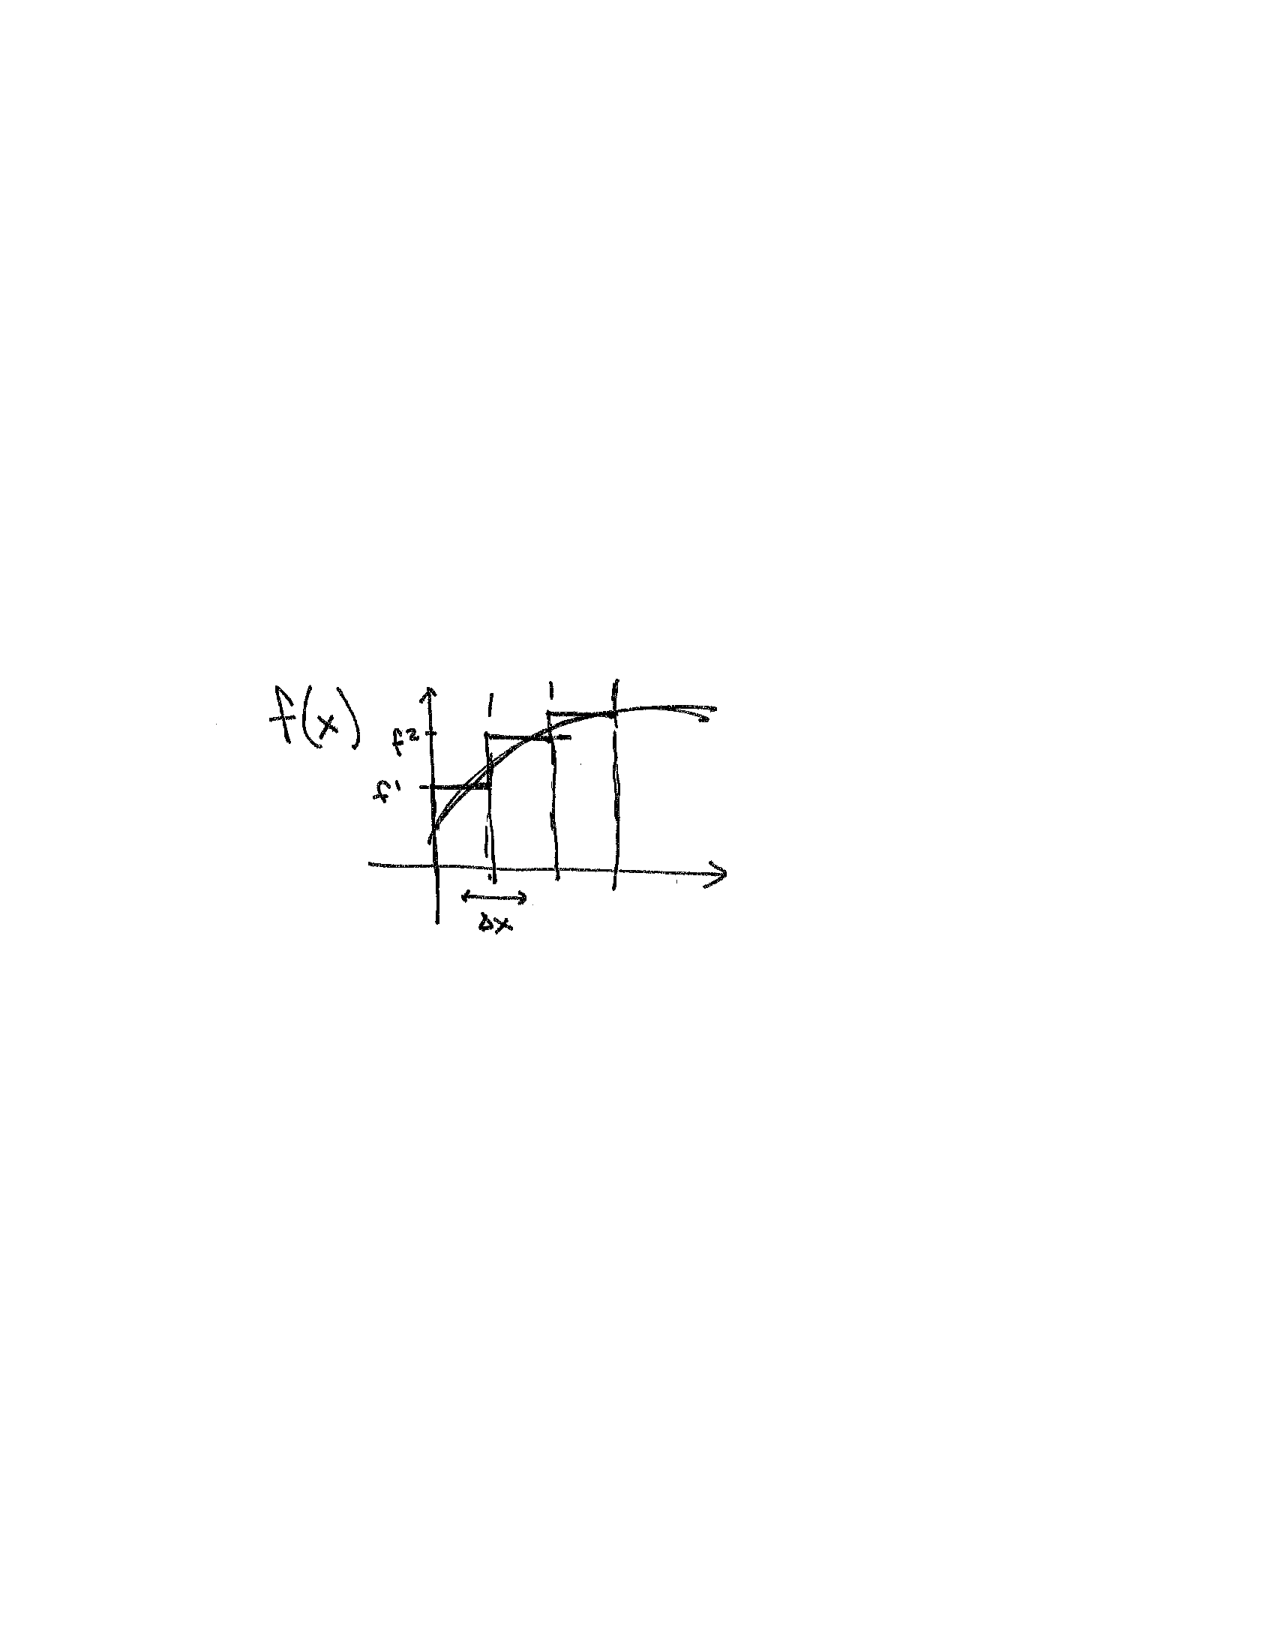
\includegraphics[width=.4\textwidth]{figures/lec02_histfun.pdf}
\end{center}

% Thus a vector in this approximate (discretized) \emph{function} space is 
% \begin{align}
%   \vec{f} = 
%   \begin{pmatrix}
%     f^1 \\
%     f^2 \\
%     \vdots\\
%     f^N
%   \end{pmatrix} \ .
% \end{align}


This discretized function space does not formally admit an $N\to \infty$ limit. The primary reason has to do with convergence, which I always thought was not the fun part of calculus. With the caveat that this space and this basis is really silly, we push forward to get some intuition for what an infinite-dimensional vector space looks like. 
%% TO INCLUDE: why the historgram basis is dumb
%% I had some good reference for this from P17
%% ... perhaps Linear Algebra done right, or Appel or Cahill...
%% ... the point was convergence.

% In what way are polar coordinates an orthonormal basis? 

\section{Derivatives as Linear Transformations}

Our discretized function space allows us to define a forward derivative\sidenote{One could have also defined a backward derivative where $(f')^i \sim f^{i}-f^{i-1}$ \ . Note that you \emph{cannot} try to make this symmetric by defining a `centered' derivative like $(f')^i \sim f^{i+1/2}-f^{i-1/2}$ because there's no such thing as a fractional index. If you tried to write $(f')^i\sim f^{i+1}-f^{i-1}$ you're making a worse approximation. If you're like me, the fact that there's some asymmetry in how we define the first derivative is deeply unsettling. There's something to this intuition!}:
\begin{align}
  \ket{f'} =
  \frac{1}{\Delta x}
  \begin{pmatrix}
    f^2 - f^1 \\
    f^3 - f^2 \\
    \vdots
    \\
    f^{i+1}-f^i
    \\
    \vdots
  \end{pmatrix} \ .
\end{align}
This is familiar if you have ever had to manually program a derivative into a computer program. Note that the right-hand side is a linear transformation of $\vec{f}$. In other words, we may write a matrix $D_+$ so that
\begin{align}
  \ket{f'} = D_+\ket{f} \ .
\end{align}
One problem is apparent: what happens at the `bottom’ of the vector? What is the last component of the derivative, $\vec{f'}^N$? Formally, this is
\begin{align}
  {(f')}^N = \frac{1}{\Delta x}(f^{N+1} - f^N) \,
\end{align}
but now we have no idea what $f^{N+1}$ is. That was never a component in our vector space. There is no $\vec{e}_{(N+1)}$ basis vector. 


We could also define a backward derivative, $D_-$,
\begin{align}
  \ket{f'} =
  D_- \ket{f}
  =
  \frac{1}{\Delta x}
  \begin{pmatrix}
    \vdots \\
    f^2 - f^1 \\
    \vdots
    \\
    f^{i}-f^{i-1}
    \\
    \vdots\\
    f^{N}-f^{N-1}
  \end{pmatrix} \ .
\end{align}
The question is now on the opposite boundary: what is the first component of $D_-\ket{f}$?


This demonstrates and important lesson that we’ll need when we move more formally to function spaces:
\begin{bigidea}
{Boundary conditions are part of the definition of the function space}.   
\end{bigidea}
That was so important that I put the whole damn sentence in boldface and set it in the middle of the line. The significance of boundary conditions may be a bit surprising---but think of this as part of the definition of which functions we allow into our function space. 
% 
There are three nice choices for boundary conditions, which we illustrate in Fig.~\ref{fig:boundary:conditions}.

%
% \begin{example}
% When one first learns about Fourier series with Dirichlet boundary conditions, one finds that the Fourier expansion \emph{only} contains sines. The solution to the wave equation in such a system is some function that is zero at each endpoint. So the function space relevant to the system is composed only of functions that are zero at each endpoint.
% \end{example}

% FIGURE SNIPPIT
\begin{figure}[tb]
    \centering
    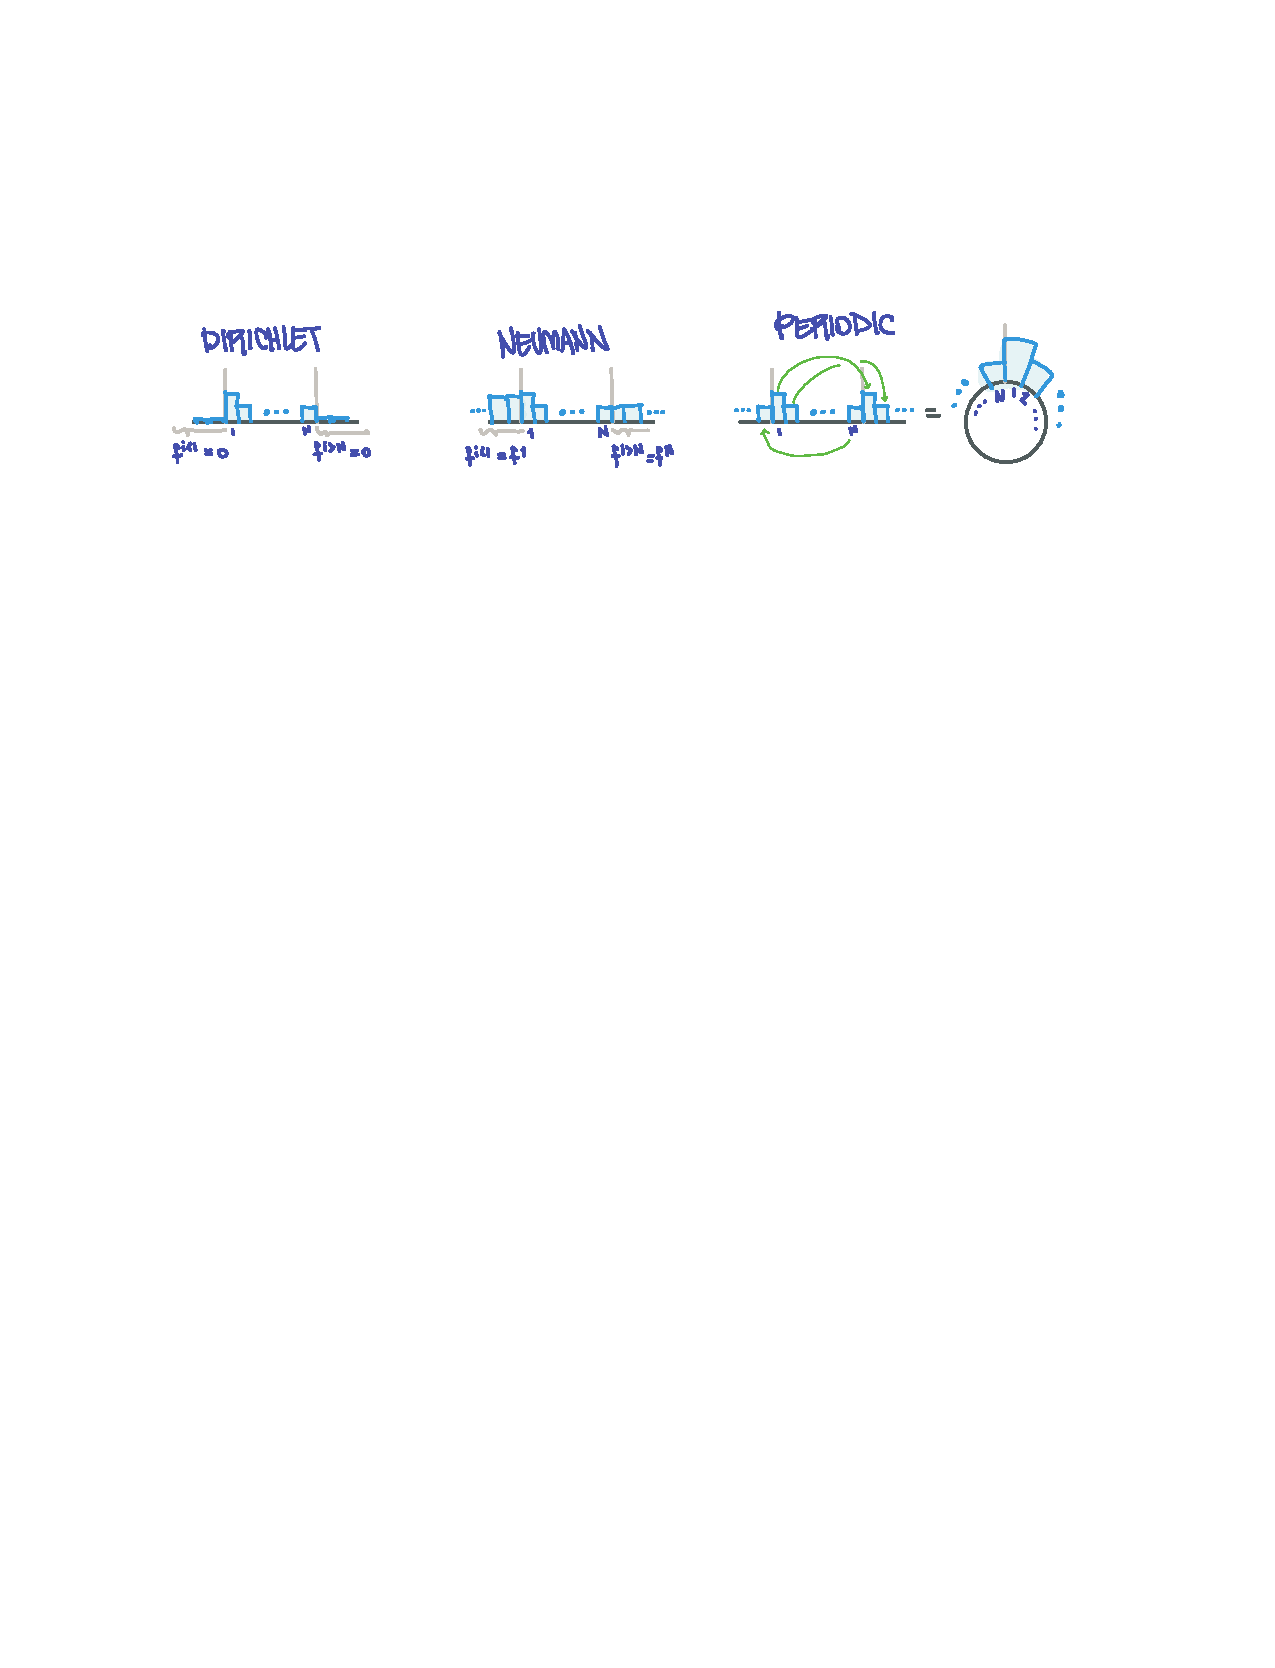
\includegraphics[width=.95\textwidth]{figures/BoundaryConditions.pdf}
    \caption{Some of our favorite boundary conditions. These are not only physically motivated, but will be important for defining Hermitian differential operators.}
    \label{fig:boundary:conditions}
\end{figure}



\paragraph{Dirichlet}
The simplest option is a \textbf{Dirichlet boundary condition}. Here we assert that the function vanishes for all of the bins below $i=1$ and above $i=N$. This choice corresponds to the following definition of what happens to all functions outside the domain of the function space:
\begin{align}
  f^{i > N} = f^{i < 1} = 0 \ .
\end{align}
This solves the problem of the derivative on the last component of $D_+$ and the first component of $D_-$:
\begin{align}
  (f')^N_\text{+, Dir.} &= \frac{f^{N+1} - f^N}{\Delta x} 
  = 
  \frac{- f^N}{\Delta x}  
  &
 (f')^1_\text{-, Dir.} = \frac{f^{1} - f^0}{\Delta x} 
  = 
  \frac{f^1}{\Delta x}
  \ .
\end{align}
\begin{example}
With Dirichlet boundary conditions, the matrix expression for the forward/backward derivative $D_\pm$ is
\begin{align}
    \left(D_+\right)_\text{Dir.}
    &=
    \frac{1}{\Delta x}
    \begin{pmatrix}
        -1 & 1 & & &  \\
        & -1 & 1 & &  \\
        & & -1 & 1 &  \\
        & & & \ddots & \ddots &  \\
        & & & & -1 & \pp 1 \\
        & & & & & -1 
    \end{pmatrix}
    \\
    \left(D_-\right)_\text{Dir.}
    &=
    \frac{1}{\Delta x}
    \begin{pmatrix}
        \pp 1 & & & &  \\
         -1 & 1 & &  \\
        & -1 & 1 &  \\
         & & \ddots & \ddots &  \\
        & & & -1 &  1 
    \end{pmatrix}
\end{align}
Observe that neither of these matrices is Hermitian in the conventional finite dimensional sense.
\end{example}


\paragraph{Neumann} Another choice for boundary conditions is that the function remains constant below $i=1$ and above $i=N$. This amounts to enforcing that the derivative vanishes at the boundaries. We call these \textbf{Neumann boundary conditions}:
\begin{align}
    f^{i<1} &\equiv f^i
    &
    f^{i>N} &\equiv f^N \ .
\end{align}
This implies that 
\begin{align}
  (f')^N_\text{+, Neu.} &= \frac{f^{N+1} - f^N}{\Delta x} 
  = 
  9
  &
 (f')^1_\text{-, Neu.} = \frac{f^{1} - f^0}{\Delta x} 
  = 
  0
  \ .
\end{align}
\begin{example}
With Neumann boundary conditions, the matrix expression for the forward/backward derivative $D_\pm$ is
\begin{align}
    \left(D_+\right)_\text{Neu.}
    &=
    \frac{1}{\Delta x}
    \begin{pmatrix}
        -1 & 1 & & &  \\
        & -1 & 1 & &  \\
        & & -1 & 1 &  \\
        & & & \ddots & \ddots &  \\
        & & & & -1 & \pp 1 \\
        & & & & & 0 
    \end{pmatrix}
    \\
    \left(D_-\right)_\text{Neu.}
    &=
    \frac{1}{\Delta x}
    \begin{pmatrix}
        \pp 0 & & & &  \\
         -1 & 1 & &  \\
        & -1 & 1 &  \\
         & & \ddots & \ddots &  \\
        & & & -1 &  1 
    \end{pmatrix}
\end{align}
\end{example}


\paragraph{Periodic} Alternatively, we could  impose \textbf{periodic boundary conditions}. This is the assumption that the boundary to the right of $i=N$ is equivalent to the boundary to the left of $i=1$. Periodic boundary conditions amount to wrapping the $x$-axis into a circle. Older folks sometimes call this \emph{Asteroids} boundary conditions:
\begin{align}
  f^{i} &= f^{i+ kN}
  & k\in \mathbb{Z} \ .
\end{align}
This gives
\begin{align}
  (f')^N_\text{$+$, Per.} &= \frac{f^{N+1} - f^N}{\Delta x}
  = 
  \frac{f^1- f^N}{\Delta x}  
  &
 (f')^1_\text{$-$, Per.} &=\frac{f^{1} - f^0}{\Delta x} 
 = \frac{f^{1} - f^N}{\Delta x} 
  \ .
\end{align}
\begin{example}
With Periodic boundary conditions, the matrix expression for the forward/backward derivative $D_\pm$ is
\begin{align}
    \left(D_+\right)_\text{Per.}
    &=
    \frac{1}{\Delta x}
    \begin{pmatrix}
        -1 & 1 & & &  \\
        & -1 & 1 & &  \\
        & & -1 & 1 &  \\
        & & & \ddots & \ddots &  \\
        & & & & -1 & \pp 1 \\
        1 & & & & & -1 
    \end{pmatrix}
    \\
    \left(D_-\right)_\text{Per.}
    &=
    \frac{1}{\Delta x}
    \begin{pmatrix}
        1 & & & &  -1\\
         -1 & 1 & &  \\
        & -1 & 1 &  \\
         & & \ddots & \ddots &  \\
        & & & -1 &  1 
    \end{pmatrix}
\end{align}
Look at those funny non-zero elements in the far corners. 
\end{example}
% \begin{align}
%   {(f')}^N = \frac{1}{\Delta x}(f^{N+1} - f^N) 
%   = 
%   \frac{1}{\Delta x}(f^{1} - f^N) 
%   \ .
% \end{align}
 Periodic boundary conditions show up \emph{all} the time in physics. Sometimes they show up in obvious places, like the Brillouin zone of a crystal lattice. Other times they show up in not-so-obvious places like the boundary conditions of the known universe. %In addition to being crucial for a well-defined function space, the boundary conditions of a system establish its topology\footnote{I cannot over-emphasize the importance of topology in contemporary physics. Most of the physics you will learn in your first year graduate courses are intrinsically \emph{local} because the laws of physics are causal. Topological quantities are \emph{global}, they are integrals over an entire space. Because winding numbers (and their higher-dimensional cousins) are quantized, they are robust against perturbations. The number of holes in a donut is one, whether or not it's been slightly squished in the box.}.

\begin{exercise}
We don't know anything about the universe outside the Hubble radius. Why do you think it would be reasonable in a physical model to \emph{assume} that it has periodic boundary conditions? Hint: what would happen to the $x$-momentum of an asteroid in the classic arcade game \emph{Asteroids} if the game did not have periodic boundary conditions? 
\end{exercise}

\paragraph{Mixed boundary conditions} You may also impose a Dirichlet boundary condition on one boundary and a Neumann boundary condition on the other boundary. 
\begin{exercise}
Write out the matrix expressions for the forward and backward derivatives $D_\pm$ with mixed boundary conditions with a Dirichlet boundary at $i=0$ and a Neumann boundary at $i=N+1$.
\end{exercise}

\paragraph{Second derivative}
The second derivative may be defined symmetrically:
\begin{align}
  (f'')^i = \frac{(f^{i+1} - f^i) - (f^i - f^{i-1})}{\Delta x^2} \ .
\end{align}
You may pontificate about the reason why the first derivative does have a symmetric discretization while the second derivative does. 
\begin{example}
We may write the second derivative in matrix form:
\begin{align}
    \begin{pmatrix}
        \ddots & & & & 
        \\
        & 1 & -2 & 1 &  & 
        \\
        &  & 1 & -2 & 1 &  \\
        &  &  & 1 & -2 & 1 \\
        & & & & &  &\ddots
    \end{pmatrix} \ .
    \label{eq:second:derivative:matrix}
\end{align}
We omit writing zeros and remain agnostic about the boundary conditions which affect the first and last rows of the matrix. Observe that the second derivative matrix is Hermitian, whereas all of our first derivative matrices are not Hermitian.
\end{example}
Like the first derivative, one must impose boundary conditions on the second derivative operator. 

\begin{bigidea}
The choice of boundary conditions is part of the definition of the function space. Every differential operator in the function space must obey the same boundary conditions. 
\end{bigidea}

\begin{exercise}
Write out the matrix form of the forward third derivative:
\begin{align}
    \left(D_+^3 f\right)^i = \frac{1}{\Delta x}\left[(D^2 f)^{i+1}-(D^2f)^i\right] \ .
\end{align}
Observe that the third derivative matrix populates elements further away from the diagonal. This is a manifestation of the non-locality of higher derivatives. In a Taylor expansion, higher derivative terms probe the behavior of function at successively further points, even though each term is evaluated at a specific point.
\end{exercise}

\begin{example}
Do you remember the first time you saw how integration by parts worked? I still remember the first time someone showed me that $(fg)' = f'g + g'f$, so we thus have $f'g = (fg)' - g'f$. Integrate both sides over the argument and use the fundamental theorem of calculus to evaluate the definite integral over a total derivative. You can also prove this in `histogram space,' i.e.\ for finite differences. Let us do this the ponderous way to see how it works:
\begin{align}
    \sum_{i=1}^N\Delta x\, (D_+f)^i g^i
    &= \sum_{i=1}^N \left(f^{i+1}-f^{i}\right)g^i
    \\
    &= \left(f^2 g^1 - f^1 g^1\right) 
        + \left(f^3 g^2 - f^2 g^2\right) 
        % + \left(f^4 g^2 - f^3 g^2\right) 
        + \cdots
        + \left(f^{N+1} g^N - f^N g^N\right) 
    \\
    &=  - f^1 g^1 
        + \left(f^2 g^1 - f^2 g^2 \right) 
        + \left(f^3 g^2 - f^3 g^3 \right) 
        % + \left(f^4 g^2 - f^3 g^2\right) 
        + \cdots
        + f^{N+1} g^N
    \\
    &= f^{N+1} g^N -  f^1 g^1   -\sum_{i=2}^N f^i\left(g^{i-1} - g^i \right)
    + f^1g^0 - f^1g^0
    \\
    &= f^{N+1} g^N -  f^1 g^0   -\Delta x\sum_{i=1}^N f^i (D_-g)^i \ ,
    \label{eq:integration:by:parst:histogram}
\end{align}
All we have done in the intermediates steps is regrouped pairs of terms that have the same $f^i$ coefficient. In the last step we were a little tricky: we added and subtracted by $f^1g^0$ so that the $f^1g^1$ term could be combined with one of those terms to fix the limits of the sum. As a result, the final line indeed samples the boundary values: $f^{N+1}g^N$ on the upper boundary and $f^1g^0$ on the lower boundary. Observe that integrating by parts over the forward derivative on $f$ leaves the backward derivative on $g$. Also observe that we have recovered the usual boundary term. Because the inital integral is a forward derivative, the forward boundary is not symmetric. 
\end{example}

\begin{exercise}
Show that the boundary term in \eqref{eq:integration:by:parst:histogram} vanishes for Dirichlet, Neumann, and periodic boundary conditions. The Neumann case is a little tricky and one has to appeal to the $i=1$ and $i=N$ terms of the sum. 
\end{exercise}

\begin{exercise} \label{ex:integrate:kinetic:term:by:parts}
If $x(t)$ is the position of a particle of mass $m$, then its kinetic term is $m\dot x(t)/2$. One way to derive the equation of motion for a theory is to integrate this term by parts, see Section~\ref{eq:variational}. Let us see how this works. Rather than $\dot x^2$, let us consider $(D_+f)(D_-g)$. We write $f$ and $g$ to make it easier to keep track of terms, but for the specific case of the kinetic term we know $f=g=x(t)$. 

The integral over time corresponds to a sum over the time slice (histogram) index $i$ of $f$ and $g$:
\begin{align}
    \int dt\, \dot x(t)^2 \to \sum_i \Delta x \, (D_+f)^i(D_-g)^i \ .
\end{align}
Show that this sum takes the form
\begin{align}
    \sum_i \Delta x \, (D_+f)^i(D_-g)^i 
    = -\sum_i f^i (D^2 g)^i 
    + f^{N+1}(g^N-g^{N-1})
    - f^1(g^1 - g^0) \ .
\end{align}
I was sloppy with the limits of the sum above. What values does $i$ range over in that sum?
% HINT:
\acro{Partial answer:}
Here's the pattern:
\begin{align}
    D_+fD_-g &= 
    f^2g^2 - f^2g^0 - f^1 g^1 + f^1 g^0\\
    &+ f^3 g^2 - f^3 g^1 - f^2 f^2 + f^2 g^1 \\
    &+ f^4 g^3 - f^4 g^2 - f^3 g^3 + f^3 g^2 \\
    &+ \cdots \\
    & + f^{N+1} g^N - f^{N+1} g^{N-1} - f^N g^N + f^N g^{N-1}  \ .
\end{align}
\end{exercise}

\section{Derivatives in other function space bases}
\label{sec:derivatives}

% \flip{This section can be skipped on a first reading.}

There are other ways to write a discrete basis of functions. Here is a natural one for functions that are up to second-order polynomials:
\begin{align}
  \ket{e_0} &= 1
  &
  \ket{e_1} &= x
  &
  \ket{e_2} &= x^2 \ .
\end{align}
Let’s sidestep questions about orthonormality for the moment. Clearly linear combinations of these basis functions can produce any quadratic function:
\begin{align}
  f(x) &= a x^2 + bx + c
  & \Rightarrow&&
  \vec{f} &=
  \begin{pmatrix}
     c \\ b \\ a
   \end{pmatrix} \ . 
\end{align}
The derivative operator has an easy representation in this space:
\begin{align}
  D = 
  \begin{pmatrix}
    0 & 1 & 0   \\
    0 & 0 & 2   \\
    0 & 0 & 0   
  \end{pmatrix} \ .
\end{align}
We can see that
\begin{align}
  D \vec{f}  &= 
  \begin{pmatrix}
     b \\
     2 a \\
     0
  \end{pmatrix} 
  &
  D^2 \vec{f}  &= 
  \begin{pmatrix}
     2a \\
     0 \\
     0
  \end{pmatrix} 
  &
  D^3 \vec{f}  &= 
  0 \ .
\end{align}
The last line is, of course, the realization that the third-derivative of a quadratic function vanishes. Feel free to attach mathy words to this like \emph{kernel}.\footnote{Unfortunately `kernel' is also used when discussing probability distributions. To the best of my knowledge the two usages are completely independent.} One hint why this basis may be annoying is that the second derivative matrix is not Hermitian, unlike in \eqref{eq:second:derivative:matrix}.

There are other bases that we may use for function space. A particularly nice one that we will use over and over is the Fourier basis, which we usually refer to as \emph{momentum space}. The basis vectors are things like sines, cosines, or oscillating exponentials. These do not vanish for any power of $D$.


\section{Locality}
\label{sec:locality}

Notice that in the histogram basis, the derivative matrix $D$ is sparse: it is zero everywhere away from the diagonal. The only non-zero elements on the $i^\text{th}$ row are around the $(i\pm 1)^\text{th}$ column.  Higher powers of $D$ sample further away, but the non-zero elements are always clustered near the diagonal.

This is simply a notion of \textbf{locality}. Remember the Taylor expansion:
\begin{align}
  f(x) = f(0) + f'(0) x + \frac{1}{2} f''(0)x^2 + \cdots \ .
\end{align}
If we think about the histogram as a discretization of a continuous function, then it is clear what the higher derivatives are doing. Given a function $f(x) = \vec{f}$, one might like to know about the function around some point $x_0$ corresponding to some index $i$. That is: $f^i = f(x_0)$. If you’d like to learn more about the function around that point, one can express the derivative at $x_0$. Thus $D\vec{f}$ says something about the slope, $D^2\vec{f}$ says something about the curvature, and so on. Because each successive power of $D$ samples terms further away from $f^i$, you can tell that these higher order terms are learning about the function further and further away from $x_0$. 

Now think about the types of differential equations that you have encountered in physics. They often include one or two derivatives. You hardly ever see three, four, or more derivatives\footnote{With some thought, it may also be clear why spatial derivatives typically appear squared.}. There is a reason for this: at the scales that we can access experimentally, nature appears to be local. Our mathematical models of nature typically have locality built in\footnote{A recent counterexample ``A Jewel at the Heart of Quantum Physics,'' by Natalie Wolchover in \emph{Quanta Magazine} (2013).
% https://www.quantamagazine.org/physicists-discover-geometry-underlying-particle-physics-20130917/
}. Physics at one spacetime point should not depend on spacetime points that are far away. 

We mentioned this in Section~\ref{eq:simultaneity} when we thought about special relativity. Recall the idea of causality---the idea that $A$ \emph{causes} $B$ therefore $A$ must have happened \emph{before} $B$. One of the key results in special relativity is that causality can be tricky if two events do not occur at the same spacetime point. More carefully, $A$ can only cause $B$ if there is a timelike separation of the appropriate sign.  If we want to build causal theories of nature, then the dynamics at $x_0$ should not rely on what is happening at $x_1$, a finite distance away.\footnote{This is different from saying that information cannot propagate from $x_0$ to $x_1$; such propagation could come from some causal excitation of the electromagnetic field traveling every infinitesimal distance between the two positions. This is reminiscent of the classical Zeno's paradox.}

% \section{The Green's Function Problem in Function Space}

% The Green's function can be defined by analogy to the finite-dimensional inverse transformation. The finite-dimensional linear system $A\vec v = \vec w$ can be solved by applying the inverse transformation $A^{-1}$ in the same way that the continuum (infinite-dimensional) system $\mathcal O \psi(x) = s(x)$ can be solved with the Green's function $G(x,y)$ of the operator $\mathcal O$:
% \begin{align}
%   v^i &= \sum_i 
%   \mat{\left(A^{-1}\right)}{i}{j} w^j
%   &\Rrightarrow
%   &
%   &
%   \psi(x) &= \int  dy\, G(x,y) s(y) \ .
%   \label{eq:def:of:function:space:Greens:function}
% \end{align}
% We've explicitly written out the sum over the dummy index $i$ to emphasize the analogy to the integration over the dummy variable $y$. The arguments of the functions play the role of `continuum indices.'


The assumption that nature is local leads to physical \emph{dynamics} that are described in terms of derivatives. Newton's law is 
\begin{align}
    m \ddot{\vec{x}} (t) = -\nabla V \ .
\end{align}
On the left hand side is a second derivative in time. The right hand side is simply a function---nevermind that it is a spatial gradient of a potential. Most of our equations of motion are written in a differential form:
\begin{align}
    \mathcal O f(x) = s(x) \ ,
\end{align}
where $\mathcal O$ is a \textbf{differential operator} that is a matrix in function space built out of derivatives, $f(x)$ encodes something about the state of the system, and $s(x)$ is a source for the dynamics. For Newton's force law, $\mathcal O = (d/dt)^2$ and $s=-\nabla V/m$. The variable is often time since we care about the time evolution of a system and our dynamical laws tell us the `small change' in a state after a `small time evolution.' More generally, it can be a spacetime position coordinate.



\section{Differential Operators}

Linear transformations on function space are differential operators. In principle you can imagine linear transformations that are not differential operators, for example a finite translation. However, because our models of nature are typically \emph{local} and \emph{causal}, the linear transformations that we obtain from physical models are differential operators\sidenote{This is not to say that finite transformations are somehow not permitted. The dynamics that govern our models of nature, however, only dictate how information is transmitted infinitesimally in space and time. Propagation forward in time by some finite interval is described by the exponentiation of infinitesimal forward time translations. This is, of course, why the time-translation operator in quantum mechanics is $e^{i\hat H t}$, where the Hamiltonian $H$ is described as a local function with perhaps one or two derivative operators.}. 

Let's write a general differential operator as:
\begin{align}
  \mathcal O = 
  p_0(x) 
  + p_1(x) \frac{d}{dx}
  + p_2(x) \left(\frac{d}{dx}\right)^2
  + \cdots
  \label{eq:differential:operator}
\end{align}
where the $p_i(x)$ are polynomials. Sometimes we will write this as $\mathcal O_x$ to make it clear that the argument of the polynomials is $x$ and the variable with which we are differentiating is $x$.  
\begin{exercise}
Explain why \eqref{eq:differential:operator} is a linear operator acting on function spaces.
\end{exercise}
\begin{exercise}
A confused colleague argues to you that \eqref{eq:differential:operator} cannot possibly be `linear.' Just look at it, your colleague says: the functions $p_i(x)$ are polynomials---those aren't \emph{linear}! There are also powers of derivatives---how is that possibly linear? Explain to your colleague why the $p_i(x)$ does not have to be linear nor is one restricted to finite powers of derivatives for the operator $\mathcal O$ to be a linear operator acting on function space.
\end{exercise}
Technically \eqref{eq:differential:operator} is called a \textbf{formal operator} because we haven't specified the boundary conditions of the function space. Recall in our discretized `histogram space' in Section~\ref{sec:histogramspace} that we had to be careful about how to define the derivative acting on the boundaries of the space. A differential operator along with boundary conditions is called a \textbf{concrete operator}.

\section{Inner Product}

Let us return to finite-dimensional histogram space. As long as we are finite dimensional, this is a perfectly legitimate vector space. We would like to endow this vector space with a metric. Perhaps the Euclidan metric? As we will see shortly, it is useful to define a metric that is proportional to the Euclidean metric by $\Delta x$, the discretization size of our histogram space:
\begin{align}
    g_{ij} &=
    \Delta x 
    \begin{cases}
    1 & \text{if } i=j \\
    0 & \text{otherwise}
    \end{cases}
    \ .
    \label{eq:metric:on:histogram:space}
\end{align}
This gives a definition for components with a lower index:
\begin{align}
    \bra{f} &= f_i\bra{i} & f_i &= \Delta x f^i \ .
    \label{eqref:histogram:row:vec}
\end{align}
The factor of $\Delta x$ makes it seem like the `row vector' or bra $\bra{f}$ is something that is born to be integrated over. \emph{As long as $N$ is finite,} the dual basis $\bra{i}$ is defined as usual, $\la i | j \ra = \delta^i_j$. The inner product of two histograms is
\begin{align}
    \la f , h \ra = f^i h^j g_{ij} = f^i h_i \Delta x = \sum_i f^i h^i \Delta x \ .
    \label{eq:metric:on:histogram:space:bracket:form}
\end{align}
If we think of $f_i = f(x_i)$ and $h^i=h(x_i)$ then the above sum is simply the discretization of the integral
\begin{align}
    \la f , h \ra = \int dx\, f(x)h(x) \ .
\end{align}
For complex functions, we generalize this a bit to include a complex conjugate on the first argument:
\begin{align}
  \langle f,h\rangle 
  =
  \int dx\, f^*(x)h(x) \ .
  \label{eq:L2:inner:product}
\end{align}
This is called the \acro{L2} inner product. Observe that this definition satisfies the metric condition for complex vector spaces \eqref{eq:complex:metric:star}, $\la f, h\ra = \la h, f \ra^* $.
\begin{example}
Wave functions in 1D quantum mechanics obey this norm. For an infinite domain, we typically restrict to square-integrable functions meaning that $|f|^2$ goes to zero fast enough at $\pm \infty$ so that the integral $\langle f, f\rangle$ is finite. 
\end{example}
Sometimes the inner product is defined with respect to a \textbf{weight} function $w(x)$:
\begin{align}
  \langle f,g\rangle_w 
  =
  \int dx\, w(x)\, f^*(x)g(x) \ .
  \label{eq:weighted:inner:product}
\end{align}
There's nothing mysterious about inner products with weights. They typically boil down to the fact that one is not using Cartesian coordinates. We will assume unit weight until we go to higher spatial dimensions\footnote{My dissertation focused on theories of extra dimensions. I also noticed that my weight increased in my final year of graduate school as I spent most of my time writing about extra dimensions and eating cafe pastries.}.
\begin{example}
Have you met the Bessel functions? If not, you're in for a treat in your electrodynamics course. The Bessel functions satisfy a funny orthogonality relation with weight $w(x)\sim x$ because they show up as the radial part of a solution when using polar coordinates. When you separate variables, $\D[2]x = r\D{r}\D{\theta}$, we see that the measure over the radial coordinate $r$ carries a \emph{weight} $r$.
\end{example}

\section{Adjoint}

This looks very promising. We have an inner product that can pave the way to taking the infinite dimensional limit of our histogram space. We can now make more precise statements about derivatives. We use the term \textbf{differential operator} (or simply operator) to mean some linear transformation built out of derivatives that act as matrices in function space. There are other `matrices'  that are not differential operators, but these tend to be \emph{nonlocal} and hence do not often show up in physical theories. We can now formalize the sense in which some differential operators are self-adjoint (Hermitian) and others are not. Recall that a self-adjoint operator satisfies \eqref{eq:self:adjoint},
\begin{align}
    \mathcal O^\dag &= \mathcal O
    &
    \text{where}&
    &
    \la \mathcal O^\dag f,h\ra \equiv \la f, \mathcal O h \ra \ .
\end{align}
Recall that we have to assume some boundary conditions for the space. 
Writing this out with respect to our integral expression for the inner product:
\begin{align}
\int dx \, \left[\mathcal O^\dag f(x)\right]^*  h(x)
&=
  \int dx \, f(x)^* \left[\mathcal O h(x)\right]
   \ .
\end{align}
The strategy is as follows: given an inner product (integral) over $f^*$ and $g$ where there is some stuff ($\mathcal O$) acting on $g$, can we re-write this as an integral with no stuff acting on $g$ and some \emph{other} stuff acting on $f^*$? If so, then the `other stuff' is the adjoint $\mathcal O^\dag$.

\begin{example}
What is the adjoint of the derivative operator, $\mathcal O = d/dx$? Assume an interval $x\in[a,b]$ and Dirichlet boundary conditions, $f(a)=f(b)=0$. There's a simple way to do this: integrate by parts.
\begin{align}
  \int dx \,  f(x) \left[\frac{d}{dx} g(x)\right]
  =
  - \int dx \, \left[\frac{d}{dx}f(x)\right]^* g(x)
  +
  \left[f^*(x)g(x)\right]^b_a \ 
  =
  \int dx \, \left[-\frac{d}{dx}f(x)\right]^* g(x)
  \ . 
\end{align}
From this we deduce that
\begin{align}
  \left(\frac{d}{dx}\right)^\dag = -\frac{d}{dx} \ .
\end{align}
\end{example}

% \begin{example}
% Consider the vector space of functions defined over $-1 \leq x \leq 1$ with Dirichlet boundary conditions. The first derivative, $\mathcal O = d/dx$, is not Hermitian. We can show this using integration by parts and the \acro{L2} inner product \eqref{eq:L2:inner:product}:
% \begin{align*}
%     \left\la \frac{d}{dx} f , h \right\ra
%     &= 
%     \int_{-1}^1 dx\, f'(x) h(x)
%     =
%     \int_{-1}^1 dx\, \frac{d}{dx}\left[f(x)h(x)\right]
%     - 
%     \int_{-1}^1 dx \, f(x) h'(x)
%     = 
%     - \left\la f, \frac{d}{dx} h \right\ra \ .
% \end{align*}
% We have used the Dirichlet boundary conditions to remove the boundary term. Observe that $(d/dx)$ is \emph{almost} self-adjoint. If only it weren't for that damn minus sign. 
% \end{example}


We will be especially interested in \textbf{self-adjoint} (Hermitian) operators for which
\begin{align}
  \mathcal O^\dag = \mathcal O \ .
\end{align}
This is, as we mentioned for the finite-dimensional case, because self-adjoint operators are \emph{nice}: they have real eigenvalues and orthogonal eigenvectors. Since most physical values are real eigenvalues of some operator, one may expect that the differential operators that show up in physics are typically self-adjoint.
\begin{exercise}
We saw above that the derivative operator is not self-adjoint. Show that the complex differential operator $\mathcal O=i(d/dx)$ is self-adjoint. \emph{Hint: what is the momentum operator in quantum mechanics?}\footnote{\url{https://aapt.scitation.org/doi/abs/10.1119/1.9932}} 
\end{exercise}


\begin{example}
Consider $\mathcal O = -(d/dx)^2$ defined on the domain $x\in [0,1]$ with the boundary conditions $f(0)=f(1)=0$. Is this operator self-adjoint? We want to check of $\langle f,\mathcal O g\rangle = \langle O f, g \rangle$. We have one trick: integration by parts. Let's see how this works.
\begin{align}
  \langle f, \mathcal O g\rangle &= - \int dx\, f^*(x)\frac{d^2}{dx^2} g(x) \ .
\end{align}
This is compared to
\begin{align}
  \langle \mathcal O f, g\rangle 
  &= -\int^1_0 dx\, \left[ \frac{d^2f}{dx^2}\right]^*g(x) 
  \\
  &= 
  -\left.
    \left(\frac{df}{dx}\right)^*
    g(x)
    \right|^1_0
  + \int^1_0 dx \, \left(\frac{df}{dx}\right)^* \frac{dg}{dx}
  \\
  &= \left.f^*(x) \frac{dg}{dx} \right|^1_0
  - \int^1_0 dx \, f^*(x) \frac{d^2g}{dx^2}  
  \\
  &=
  - \int^1_0 dx \, f^*(x) \frac{d^2g}{dx^2}
  \ .
\end{align}
And so we see that indeed $(-d^2/dx^2)^\dag = -d^2/dx^2$.
\end{example}
\begin{exercise}
In the previous example, what is the significance of the overall sign of the operator? \emph{Hint: the sign doesn't matter, it's because we typically think of $-\partial^2$ and its higher-dimensional derivatives as the square of the momentum operator.}
\end{exercise}
\begin{example}\label{ex:eigenfunction:fourier}
The \textbf{eigenfunctions} $f_n$ of $-d^2/dx^2$ defined on $x\in [0,1]$ with Dirichlet boundary conditions are simply 
\begin{align}
  f_n(x) &= A_n \sin(n\pi x) 
  &
  \lambda_n = n^2\pi^2 \ ,
  \label{eq:fourier:basis:unit:interval}
\end{align}
where $\lambda_n$ is the associated eigenvalue and $A_n$ is some normalization that. These eigenfunctions are orthonormal in the following sense:
\begin{align}
  \langle f_n, f_m\rangle = \int_0^1 dx\, \sin(n\pi x)\sin(m\pi x) = \frac{A_nA_m}{2} \delta_{nm} \ ,
\end{align}
from which we deduce that the normalization is $A_n = \sqrt{2}$. That's basically all there is to know about Fourier series.
\end{example}
\begin{exercise}
What would change if we had instead assumed Neumann boundary conditions? What if we had assumed periodic boundary conditions? What about anti-periodic boundary conditions?
\end{exercise}
\begin{exercise}\label{exe:eigenfunction:fourier}
A function $g(x)$ defined on an interval $x\in [0,1]$ with Dirichlet boundary conditions can be written with respect to the Fourier basis \eqref{eq:fourier:basis:unit:interval}. In ket notation, the $n^\text{th}$ component of $g$ with respect to this basis is
\begin{align}
  g^n = \langle f_n| g\rangle \ .
\end{align}
Confirm that this is precisely what you know from Fourier series. In other words, we can decompose $g(x)$ as
\begin{align}
  g(x) &= \sum_n \langle f_n| g\rangle f_n(x)  \ .
\end{align}
\end{exercise}





% \begin{example}
% Show that the  differential operator $\mathcal O=(d/dx)^2$ is self-adjoint. 
% \end{example}


With a clean definition of self-adjointness, we can now define `nice' differential operators are those operators that are self-adjoint. This is the function space equivalent of symmetric matrices in real, finite dimensional vector spaces and Hermitian matrices in complex, finite dimensional vector spaces. In the histogram basis we have some semblance of Hermiticity, but we saw that the $N\to\infty$ limit is a little tricky. $i(d/dx)$ is a self-adjoint operator in function space, but its discretization, the forward/backward derivative $D_\pm$, is not Hermitian because the two non-zero elements on each row are cannot be evenly spaced about the diagonal. 

The following observations carry over from finite-dimensional vector space:
\begin{enumerate}
    \item The eigenvectors of a self-adjoint differential operator are orthogonal and may be chosen to be orthonormal.
    \item The eigenvalues of a self-adjoint differential operator are real.
\end{enumerate}
The proof of these assertions are the same since they depend on general properties of the inner product. There is an additional feature: the eigenvalues are ordered. Function space is infinite in two senses: first the domain may be infinite, $x\in [-\infty, \infty]$. Second, the number of points in any finite interval is also infinite: $\Delta x \to 0$. Rather than having to discover an infinite number of eigen-stuff, we will often have \emph{one} eigenvalue equation with multiple enumerable solutions and whose eigenvalues are enumerated with respect to these solutions. 
\begin{example}
Consider the solution to the function space eigenvalue problem in Example~\eqref{ex:eigenfunction:fourier}. The eigenvalues are $\lambda_n=n^2\pi^2$ with corresponding eigenfunctions proportional to $\sin(n\pi x)$. The integer $n$ enumerates the solution and plays role of the index of the eigenbasis.
\end{example}

Finally, we remind ourselves that we have restricted our study to `matrices' in function space that are differential operators. It is entirely possible to conceive of a matrix that is not a differential operator. The discussion of locality in Section~\ref{sec:locality} motivates that \emph{physical} theories are local and hence the dynamical equations of motion are written with respect to differential operators. Similarly, matrices are usually uniform across all of space: this is because of the physical principle of translation invariance. The laws of physics in one location are the same laws as they are at another location in both space and time. This does not mean that the \emph{source} of a physical effect is uniform, only that the \emph{dynamics} are uniform. 

At this point one should review Section~\ref{sec:inverting:nice:matrices}. The general form of an eigenfunction problem in physics is that we are given some \emph{equation of motion}
\begin{align}
    \mathcal O f(x) = s(x) 
\end{align}
that describes what happens to a \emph{state} $f(x)$---perhaps the position of a particle---under some \emph{dynamics} described by the differential operator $\mathcal O$ whose effects are\emph{sourced} by $s(x)$. If $\mathcal O$ is self-adjoint, then we can diagonalize it with respect to an eigenbasis and solve this problem trivially. Most of the named special functions that show up in physics are only name-worthy because they are eigenfunctions of differential operators that show up in physics.





\section{Cracks in the scaffolding as we go to the continuum}

The \textbf{Fourier} basis and its generalizations describe function space with basis vectors that are in a sense maximally delocalized. In the example of a one dimensional interval $x\in[0,L]$ with Dirichlet boundary conditions---Example~\ref{ex:eigenfunction:fourier}---the Fourier basis were functions with a \textbf{spectrum} of wave numbers, $k_n$:
\begin{align}
    f_n(x) &= \sqrt{\frac{2}{L}} \sin(k_nx)
    &
    k_n &= \frac{n\pi}{L} \ .
    \label{eq:example:of:fourier:basis}
\end{align}
Aside from nodes, the basis functions are non-zero across all of the domain, $x\in [0,L]$. This is in stark contrast to the `position basis,' which I have deliberately not tried to define rigorously, but have instead pointed to a limiting case of the histogram basis where $\Delta x \to 0$. The histogram basis vectors are totally localized. As a useful bit of nomenclature: physicists usually refer to the Fourier basis as \textbf{momentum} states in contrast to the position eigenstates of the histogram basis. 


Something goes wrong as we formally pass from the histogram basis to a continuum basis. That is, when we take the $N\to \infty$ limit.\footnote{There are two $N\to \infty$ limits: the first one is the infinite number of points in any finite interval. The second is the infinite size of a space whose boundaries go to $\pm\infty$. } The notion of building up continuous functions $f(x)$ from the histogram basis above is problematic from the point of view of mathematical rigor. You can read more about the problems in Appel, \emph{Mathematics for Physicists} Chapter 9.1 (``Insufficiency of Vector Spaces''), or Hassani, \emph{Mathematical Physics}, Chapter 7 (``Hilbert Spaces''). As long as histogram space is finite dimensional, you can treat it as $\RR^N$ and even endow it with an inner product---say the Euclidean inner product. If you want to be fancy, at this level the metric space in the $N\to\infty$ limit is called a \emph{pre-Hilbert} space. 


\subsection{Inner Product Pickle}

One problem that shows up is that the norm of a vector is now an infinitely long series. If we had not inserted the $\Delta x$ in our definition of the metric \eqref{eq:metric:on:histogram:space}, then the norm of a function in histogram space would be
\begin{align}
    |f|^2 = \la f, f \ra = \sum_{i=1}^\infty (f^i)^2 \ .
    \label{eq:norm:in:function:space:no:dx}
\end{align}
How do you normalize a vector that has $f^i = 1$ for all values of $i$? Enforcing $|f|^2 = 1$ seems to imply that each $f^i \to 0$. This is very fishy.  Inserting the $\Delta x$ in the metric---as we did in \eqref{eq:metric:on:histogram:space:bracket:form}---seems to help:
\begin{align}
    |f|^2 = \sum_{i=1}^\infty (f^i)^2 \Delta x \to \int dx\, |f(x)|^2 \ .
    \label{eq:norm:in:function:space}
\end{align}
If the interval on which our function is defined has length $L = x_\text{max}- x_\text{min}$, then we may enforce that $\Delta x = L/N$ so that the discrete sum makes sense as $N\to\infty$. On the right-hand side we take the continuum limit. Functions for which the integral over $|f(x)|^2$ are well-defined\footnote{This means that they are non-zero and do not diverge.} are known as \emph{square integrable}, or \acro{L2}. 

\subsection{Bras as distributions}

Let us try to make sense of the basis bras. We know from Section~\ref{sec:machine:to:make:row:vectors} that the inner product gives us a natural way to define bras from kets. In the finite dimensional limit, we had  $\bra{f}$ with components $f_i\equiv \Delta x f^i$, see \eqref{eqref:histogram:row:vec}. The factor of $\Delta x \to dx$ makes it clear that the bras of function spare are \emph{distributions}: functions that are born to be integrated over.\footnote{In probability theory we write the probability distribution of a continuous variable to be $p(x)\,dx$. The interpretation is that the probability to find $x\in (a,b)$ is the integral $\int_a^b dx\, p(x)$. The value of $p(x)$ by itself does not mean anything: it is the probability that $x$ is \emph{exactly} some value, say $x=1.00000$ and not $x=1.00001$.} The inner product tells us that the bra $\bra{f}$ is
\begin{align}
    \bra{f} = \la f, \smallslot \ra   = \int dx\, f(x)^* \smallslot \ .
\end{align}
Just feed it a function (ket) and perform the integral. We have left the limits of integration implicit, but we should remember that these are integrals over the domain of the function. The definition of this domain and the boundary conditions are part of the definition of the function space. 
\begin{example}
Let $ \bra{p}=\int_0^1 dx\, p(x)\smallslot$ be the probability function for some variable $x \in [0,1]$. The expectation value for some function $\ket{g}=g(x)$ is
\begin{align}
\la g\ra_p \equiv
     \la p, g \ra = \int_0^1 dx\, p(x)\,g(x) \ .
\end{align}
\end{example}

\subsection{Normalizing the Basis... something has to give}

The histogram basis $\ket{x}$ satisfies
\begin{align}
    \la x | y \ra = \la x, y \ra = 0 \quad \text{if } x\neq y \ .
\end{align}
However, in the \emph{infinite dimensional} (continuum function) limit, we can no longer say that $\la x | y \ra = 1$ if $x=y$. This is a consequence of the unusual normalization we noticed in \eqref{eq:norm:in:function:space}. Let us assume that the domain of the function space is $x\in [0,N\Delta x]$. In the histogram basis where space is discretized, we can define the basis functions as follows:
\begin{align}
    \ket{i} = 
    e_i(x) \equiv 
    \mathcal N
    \begin{cases}
    0 &\text{if } x< (i-1)\Delta x\\
    1 &\text{if } (i-1)\Delta x \leq x \leq i\Delta x\\
    0 &\text{if } \leq i\Delta x < x 
    \end{cases}    \ .
\end{align}
We have defined our histogram space as as a stepwise functions on a continuous space so that we could use the integral representation of the inner product. That looks more complicated than it needs to---this is simply a functional form of the histogram basis we introduced in Section~\ref{sec:histogramspace}. In anticipation of issues with normalizability, we have pulled out a to-be-determined normalization factor. What is the value of this normalization, $\mathcal N$? 

\paragraph{Finite dimensional intuition}
From the perspective of a finite dimensional vector space, we would like
\begin{align}
    \la i,f\ra = f^i = f(x_i) \ .
    \label{eq:finite:dim:intuition:for:Hilbert}
\end{align}
For the interval $[0,N\Delta x]$, we define $x_i = i\Delta x$. However, we should recall the factor of $\Delta x$ that we inserted in \eqref{eq:metric:on:histogram:space:bracket:form}. 
Given our normalization of the inner product, this means that we actually end up with:
\begin{align}
    \la i, f\ra = \int dx\, e_i(x)\, f(x) = \mathcal N \Delta x f(x_i) \ .
    \label{eq:basis:normalization:of:function:space}
\end{align}
We recover our desired relation \eqref{eq:finite:dim:intuition:for:Hilbert} when we pick a normalization $\mathcal N = 1/\Delta x$. The continuum limit corresponds to $\Delta x \to 0$, which means that the normalization $\mathcal N$ of the basis ket $\ket{i}$ blows up. Oh dear. 

\paragraph{Normality of basis vectors} Maybe you are braver than I am and are willing to accept that the position basis states must have infinite normalization. Indeed, this turns out to be what we will have to accept. However, that alone does not resolve all of our problems. We picked the position basis normalization $\mathcal N$ so that $\la i, f\ra$ made sense. This means that there is no more freedom to see what happens to the norm of a basis vector:
\begin{align}
    |e_i(x)|^2 = \la i , i \ra = \Delta x \mathcal N^2 = \frac{1}{\Delta x}.
\end{align}
What annoyance! We `normalized' our basis vectors in \eqref{eq:basis:normalization:of:function:space}, only to find that they are absolutely not normalized in the usual sense, $\la i, i \ra = 1$. 




% Note that we really are stuck with this: motivated by the normalization choices in \eqref{eq:norm:in:function:space} and \eqref{eq:norm:in:function:space:no:dx}, we decided that there should be a $\Delta x$ in our definition of the inner product to make the passage to the continuum limit make sense in the $\Delta x \to 0$ limit. In \eqref{eq:basis:normalization:of:function:space} it is that same factor of $\Delta x$ that has reappeared to haunt us wen trying to make sense of the height $\mathcal N$ of each ``histogram bin'' $\ket{i} = e_{i}(x)$. This gets even worse when we consider the orthonormality of these basis vectors,
% \begin{align}
%     \la i , j \ra = \int dx\, e_i(x)e_j(x) = \mathcal N^2 \Delta x \delta^i_j \ .
% \end{align}
% This diverges in the $\Delta x \to 0$ when $N\mathcal \Delta x^{-1}$. It appears that we are stuck and something has to give. What we end up sacrificing is the normality of the histogram basis vectors.






% From Shankar p.58
\paragraph{Completeness and the Dirac $\delta$-function} We can gain more insight on this by using the \textbf{completeness} relation. Earlier we called this \emph{multiplication by one}: $\one = \sum_i \ket{i}\bra{i}$. For a continuous function space this sum becomes an integral:
\begin{align}
    \int dx \, \ket{x}\bra{x} = \one \ .
    \label{eq:completeness:continuum}
\end{align}
where we have again left the integration limits implicit. If we act on a function with this representation of the identity, we have:
\begin{align}
    \ket{f} = \int dx\, \ket{x}\bra{x} f\ra  \ .
    \label{eq:function:space:completeness:ket}
\end{align}
The significance becomes more clear if we apply $\bra{y}$ to both sides:
\begin{align}
    f(y) =  \la y | f \ra = \int dx\, \la y | x \ra \la x | f \ra 
    = \int dx\, \la y | x \ra f(x) \ .
\end{align}
This tells us that whatever $\la y | x\ra$ is, it must be a distribution such that when it is integrated over $f$ it picks out the the value of $f$ at position $y$. Let us \emph{define} this object $\delta(x-y) \equiv \la y | x \ra$:
\begin{align}
    \la y | x \ra &\equiv \delta(x-y) 
    &
    \int dx\, \delta(x-y) f(x) &\equiv f(y) \ .
\end{align}
This object is called the Dirac $\delta$-function and is the function space analog of the Kronecker $\delta$. We have assumed that $\delta$-function only depends on the difference $|x-y|$. In principle it could have depended on $x$ and $y$ separately, but we know that it is only non-zero when $x=y$. Furthermore, the $\delta$-function is normalized:
\begin{align}
    \int dx\, \delta(x) = 1 \ ,
 \end{align}
 assuming that the integration region includes $x=0$. Note that $\delta(0)$ is divergent. It seems to be infinite, reflecting the $\Delta x\to 0$ limit that worried us below \eqref{eq:basis:normalization:of:function:space}.  This means that the $\delta$-function is not really an admissible ``function.'' It is not a basis vector. $\delta(x-y)$ is simply a way to make sense of the object $\la y | x\ra$. Because this object always shows up under an integral, we never have to worry about what it means at an individual point. In other words: if you ever have a $\delta$-function without a corresponding integral, you have almost certainly done something wrong. 

 \begin{exercise}
 How do you make sense of the derivative of a $\delta$-function? Hint: integrate by parts. 
 \end{exercise}
 



\begin{example}
One can vaguely motivate the $\delta$-function as the unit matrix by appealing to the `histogram basis' of discretized function space. In an ordinary finite-dimensional vector space, unit matrix can be written as
\begin{align}
  \mathbbm{1} = |1\rangle\langle 1 | + |2\rangle\langle 2 | + \cdots
  = \sum_{i,j}\delta_{i}^j|i\rangle\langle j| \ .
\end{align}
The Dirac $\delta$-function in histogram space is analogous to
\begin{align}
  \delta(x-x') &\to \delta_{x}^{x'}|x\rangle\langle x'| \ ,
\end{align}
where $x$ and $x'$ are discrete bins on the right-hand side. Thus for a discretized function $f = f(x_1)|x_1\rangle + f(x_2)|x_2\rangle + \cdots$, one has
\begin{align}
  \int dy\, \delta(x-y) f(y) = f(x) \longrightarrow \sum_j \delta_{x_j}^{x_i}|x_i\rangle\langle x_j| f\rangle  =  f(x_i) |x_i\rangle\ .
\end{align}
\end{example}




\begin{bigidea}
The issue of a normalized basis in an infinite dimensional vector space is the difference between the Kronecker $\delta$ and the Dirac $\delta$-function. The Kronecker $\delta$ is always finite: it is zero most places, and one in a small window where two discrete indices match. The Dirac $\delta$-function is zero almost everywhere, except for a single point (vanishing width) where it is formally infinite.
\end{bigidea}






% \subsection{Dual Vectors}

% What are the `dual functions' (dual vectors, bras) in function space? These are linear functions on act on functions and spit out numbers. These are integrals that are pre-loaded with some factors. Assuming unit weight:
% \begin{align}
%   \langle f | = \langle f, \qquad \rangle
%   = 
%   \int dx \, f^*(x) \left[\text{ insert ket here }\right] \ .
% \end{align}








\subsection{Completeness and Orthogonality for Countable Bases}
% This is confusing.... integral vs sum depends on countable vs noncountability of basis

In the previous subsection our ``multiplication by one'' over the histogram basis took the form of an integral, \eqref{eq:completeness:continuum}. This is a consequence of the unusual nature of the position basis. Contrast this to the Fourier (``momentum'') basis example in \eqref{eq:example:of:fourier:basis}. Both bases are infinite, as appropriate for the infinite dimensional space. However, the histogram basis is \emph{uncountable}. 

The Fourier basis is countable because we had an index, $n$, and could enumerate each of the vectors. The position basis is uncountable because given the $i^\text{th}$ basis vector, there is no notion of what the $(i+1)^\text{th}$ vector should be. What comes after $x=2.538$? $x=2.539$? What about $x=2.5385$? The countability of the Fourier basis returns us to the case of having a discrete basis, which allows us to much of the technology of \emph{finite} dimensional vector spaces.\footnote{Sometimes we are stuck with uncountable bases. The countability of the Fourier basis depends on the finiteness of the interval on which the functions are defined. When you describe the entire real line, $\RR$, in the momentum basis, you end up with basis vectors that can take continuous values of the wave number, $k$. In that case, we go between an uncountable position basis and an uncountable momentum basis. This is called a Fourier transform.}

Let us see how completeness and orthogonality work for \emph{countable} bases of infinite dimensional metric spaces.  You can write any state $|f\rangle$ with respect to the countable basis $|i\rangle$---the components are simply
\begin{align}
  f^i = \langle i | f \rangle
\end{align}
so that 
\begin{align}
  |f\rangle = \sum_i |i\rangle \langle i | v \rangle \ ,
  \label{eq:completeness:by:inserting:1}
\end{align}
which we recognize as nothing more than `multiplying by the identity.' 
%
What does completeness look like in function space?
% \begin{framed}\noindent
Let $e_{(n)}(x)$ be a set of countable basis functions. For example, $e_{(n)}(x)$ may be sines in Example~\ref{ex:eigenfunction:fourier}, but not the $\Delta x\to 0$ limit of the histogram basis.  The countable basis is \textbf{complete} if
\begin{align}
  \sum_n \left[e_{(n)}(x)\right]^* e_{(n)}(y) = \delta(x-y) \ .
  \label{eq:function:space:completeness}
\end{align}
Observe that this is an infinite \emph{discrete} sum, rather than a continuous integral as we had for the uncountable basis, \eqref{eq:completeness:continuum}.
% \end{framed}
Compare this \emph{very carefully} with the finite dimensional completeness relation, $\mathbbm{1} = \ket{i}\bra{i}$. The $\mathbbm{1}$ has been replaced by a Dirac $\delta$-function, $\delta(x-y)$. Let's confirm that this makes sense. The \emph{multiply by one} completeness relation \eqref{eq:completeness:by:inserting:1} in function space is
\begin{align}
  |g\rangle 
  &= 
  \sum_n |e_{(n)}\rangle\langle e_{(n)}| g\rangle
  &
  \langle e_{(n)}| g\rangle &=
  \int dy \, [e_{(n)}(y)]^* g(y) \ .
\end{align}
We have deliberately changed the name of the integration variable to $y$ to avoid confusion. This variable is simply a \emph{dummy variable} to be integrated over;  it doesn't matter what we name it.\footnote{By the way, this should ring a bell from our summation convention. When an upper and lower tensor index are contracted, the resulting object behaves as if it didn't have those indices: $\mat{A}{i}{j}v^j$ behaves as a vector with one upper index.} Writing this out explicitly as functions:
\begin{align}
  g(x) &= \sum_n\left[\int dy\, e_{(n)}^*(y)g(y)\right] e_{(n)}(x) \ .
  \label{eq:complenesss:function:space:in:action }
\end{align}
The factor in the square brackets is simply $\langle e_{(n)}| g\rangle$, which is just a \emph{number}---it has no functional dependence on $x$.
If this seems unusual, please refer back to Example~\ref{ex:eigenfunction:fourier} and Exercise~\ref{exe:eigenfunction:fourier}. 

% By the way, you'll often hear people (perhaps even me) say that the Dirac $\delta$ function is not strictly an \emph{function} but rather a \textbf{distribution}---this means that it only makes sense when it is integrated over. As physicists we'll sometimes be sloppy and talk about physical quantities that could be Dirac $\delta$-functions. There is \emph{never} an appropriate, measurable physical quantity that is described by a $\delta(x)$. Anything with a $\delta(x)$ is an object that was meant to be integrated over. When you imagine that a point charge density is a $\delta$-function, this is only because you will eventually integrate over it to determine the total charge.  If you ever calculate a \emph{measurable} quantity to be $\delta(x)$ check your work. If you ever find $\delta(x)^2$, then go home, it's past your bed time.

% ****
% \subsection{Orthonormality in Function Space}

One should contrast the notion of completeness of a countable basis this with that of \textbf{orthonormality} of the basis. Orthonormality is the statement that
\begin{align}
  \langle i | j \rangle = \delta^j_i \ .
\end{align}
Completeness has to do with the `outer product' $|i\rangle \langle i|$ while orthonormality has to do with the `inner product' $\langle i | i\rangle = \langle i, i\rangle$. The function space generalization of orthonormality is\footnote{If you're a purist, you'll note that $\delta_{nm}$ should really be written as $\delta^n_m$ because the dual basis vector has an upper index. While this may be true, I'm making the present notational choice because the object that we would call $\tilde{\vec{e}}^{(n)}$ really does contain $e_{(n)}^*(x)$, the complex conjugate of $e_{(n)}(x)$.}
\begin{align}
  \langle e_{(n)} | e_{(m)} \rangle = \int dx \, e_{(n)}^*(x) e_{(m)}(x) = \delta_{nm} \ .
  \label{eq:function:orthonormality}
\end{align}
\begin{exercise}
Why does \eqref{eq:function:orthonormality} have a Kronecker $\delta$ with discrete indices when \eqref{eq:function:space:completeness} has a Dirac $\delta$? Please make sure you can answer this; it establishes the conceptual foundation of the analogy between finite- and infinite-dimensional vector spaces.
\end{exercise}
For the completeness relation, we sum over the same eigenfunction label $n$ for a function and its conjugate evaluated at different continuous positions. For the orthonormality relation, we integrate over the positions of two different eigenfunction indices, $n$ and $m$. 

% Do not confuse the eigenfunction label with the index of a vector. If this is confusing, please refer back to Exercise~\ref{ex:completeness:for:non:cartesian:basis}. You may be stuck thinking about basis vectors in the Cartesian basis---this is the analog of thinking about basis functions in the `histogram basis' of Section~\ref{sec:histogramspace}. What we want to do is generalize to more convenient bases, like the eigenfunctions of differential operators (e.g.~the Fourier basis for $-d^2/dx^2$).

\begin{example}
In the case of a finite interval, say $x\in [0,1]$, the space of functions on this interval is continuous. In fact, we wrote a nice eigenbasis of $-d^2/dx^2$ on this space assuming Dirichlet boundary conditions. The basis consists of a discrete but infinite number of eigenfunctions. The discrete index, $n$, corresponded to the wave number (or momentum). The continuous `index,' $x$, corresponded to a position-space location. This index is continuous because there is a continuum of positions $x$ in the finite interval $[0,1]$. If we extended the interval to the infinite real line, $\mathbbm{R} = [-\infty, \infty]$, then the discrete spectrum of eigenfunctions---that is, the discrete separation of wave numbers---also becomes a continuum. Here the discrete spectrum of `particle in a box' states turns into a continuum of plane waves, $e^{ipx}$. 

A sufficiently large box $[-L,L]$ is approximately the same as an infinite interval. Of course, `large $L$' is a dimensionful statement. What we really want to say is that if we are probing dynamics on a scale much smaller than $L$, then we should expect the discrete spectrum of states to be so close to each other that it is well approximated by the continuum of plane waves. 

You can twist this around in the other direction and wonder if spacetime were not actually continuous but rather composed of discrete points with some spacing on the order of the Planck length. Our continuum formalism of general relativity should be valid as long as we do not ask questions about length scales comparable to the separation between discrete points. 
\end{example}

% \subsection{Fourier Series}

% Recall that the \textbf{Fourier Series} is a basis of sinusoidal functions over a finite domain. One changes variables from position $x$ to momentum or wave-number $p$. For an interval from $x\in [0,1]$, the Fourier series a function $f(x)$ with Dirichlet boundary conditions is:
% \begin{align}
%   f(x) &= \sqrt{\frac{2}{L}} 
%   \sum_{p \in \mathbb{Z}}  
%   \tilde f_p \sin(\pi p x/L) \ .
% \end{align}
% The eigenfunctions $e_p(x)=\sqrt{2/L}\sin(\pi p x/L)$ satisfy the boundary conditions and are normalized so that $\langle e_p,e_p\rangle = 1$. The data of the function $f(x)$ is encoded in an infinite number of coefficients, $\tilde f_p$.

% Fourier transforms are a basis of sinusodial functions---conventionally written as complex exponentials---over an \emph{infinite} domain. Our conventions for Fourier transforms are summarized in Appendix~\ref{app:Fourier}. 

% In statistics and machine learning, this is related to the idea of a \textbf{kernel}\index{kernel}. Kernels are the `heart' of an integral transformation that takes a function $f(x)$ to a transformed function $\tilde f(p)$ by
% \begin{align}
%   f(x) \to \tilde f(p) \equiv \int dp\, f(x) K(x,p) 
% \end{align}
% with the appropriate limits of integration. Observe that the transformed function $\tilde f$ is formally a function of a different variable. 

% \begin{exercise}
% What is the kernel of the Fourier transform using our conventions?
% \end{exercise}






\subsection{Why histogram space is dumb}
\label{sec:histogram:space:is:dumb}

% \flip{This section can be skipped on a first reading.}



There is a more formal sense in which the $N\to\infty$ limit of histogram space is challenging. This is the notion of convergence. Imagine a \emph{sequence} of vectors. This is just a list of vectors. Let us label these vectors as $\ket{v}_{(i)}$, where $i$ indexes vectors in the sequence. For example,
% example from Appel Ch. 91
\begin{align}
    \ket{v}_{(1)} &=
    \begin{pmatrix}
        1 \\ 0 \\ 0 \\ \vdots \\ 0
    \end{pmatrix}
    &
    \ket{v}_{(2)} &=
    \begin{pmatrix}
        1 \\ 2^{-1} \\ 0 \\ \vdots \\ 0
    \end{pmatrix}
    \ket{v}_{(3)} &=
    \begin{pmatrix}
        1 \\ 2^{-1} \\ 2^{-2} \\ \vdots \\ 0
    \end{pmatrix} \ .
    \label{eq:Appel:eg:cauchy:i}
\end{align}
We have chosen this sequence such it has a limiting form, $\ket{v}_{(\infty)}$
\begin{align}
    \ket{v}_{(\infty)} &=
    \left.
    \begin{pmatrix}
        2^{-0} \\ 2^{-1} \\ 2^{-2} \\ \vdots \\ 2^{-N}
    \end{pmatrix}
    \right|_{N\to\infty} \ .
    \label{eq:Appel:eg:cauchy:N}
\end{align}
We say that the sequence $\{|\ket{v}_{(i)}\}$ is a \textbf{Cauchy sequence} that limits to $\ket{v}_{(\infty)}$ if 
\begin{align}
    \lim_{i\to\infty} \ket{v}_{(i)} \to \ket{v}_{(\infty)} \ ,
\end{align}
by which we mean that the norm $|\ket{v}_{(i)}-\ket{v}_{(\infty)}|\to 0$.  The example sequence in \eqref{eq:Appel:eg:cauchy:i} has finite \emph{support}\footnote{Here the support of a vector means the non-zero elements.}, and so each element is normalizable. If we want to hold on to this notion of normalizabliity, then we may want to take our infinite-dimensional vector space and restrict to only those vectors with finite support. However, the vector $\ket{v}_{(\infty)}$ clearly does not have finite support. We say that the space of finite support vectors is not \textbf{complete} because there are Cauchy sequences that do not contain their limits.
\begin{exercise}
(From Appel, Section 9.1) Show that the sequence \eqref{eq:Appel:eg:cauchy:i} is a Cauchy sequence that converges to \eqref{eq:Appel:eg:cauchy:N}. As an intermediate step, show that
\begin{align}
    |\ket{v}_{(i)}-\ket{v}_{(\infty)}| = \sum_{j=i}^\infty \frac{1}{4^i}
    = \left(\frac{4}{3}\right)\frac{1}{4^i} \to 0 \ .
\end{align}
In the penultimate step you can use the expression for a geometric series.
\end{exercise}

The observation here is that infinite-dimensional metric spaces are not always complete. When they are complete, the metric space is called a \textbf{Hilbert space}. The great thing about Hilbert spaces is that we can treat them as $N\to\infty$ limits of finite dimensional vector spaces. 


% Another Example: Hassani Example 7.1.5 on p.217. Takes a sequence of continuous functions that limits to a discontinuous function. 



% The problem in an infinite dimensional vector space is that one can take a convergent sequence of vectors whose limiting vector is not part of the vector space. This has to do with the definition of a norm of a vector with an infinite number of terms. Our histogram space is a vector space with a good inner product: this is called a \textbf{pre-Hilbert space}. An infinite dimensional vector space that \emph{does} contain all of its limits\footnote{Formally this means that any sequence of points that progressively become arbitrarily close to each other (a Cauchy sequence) converges to a point that is also in the space.} (it is complete) is called a \textbf{Hilbert space}.

% \flip{To do: show why the histogram space fails the Cauchy sequence test.}




\subsection{Legendre Polynomials: salvaging the polynomial basis}

% \flip{This section can be skipped on a first reading.}

Consider functions on the domain $x\in[-1,1]$ with the standard function space inner product, \eqref{eq:L2:inner:product}. We now have a few reasons to think that the basis of monomials \eqref{eq:polynomial:basis} is silly. First, they do not obey an obviously meaningful boundary condition: the functions are $1$ at $x=1$  and $\pm 1$ at $x=-1$ depending on whether the index of the basis function is even or odd. It is also clear that linear combinations of these basis functions do not satisfy the same boundary conditions. Secondly, this basis behaves poorly under derivatives. Derivatives act as projection operators onto successively smaller subspaces. Finally, the monomials are not orthonormal in any meaningful sense. For example,  in the basis
\begin{align}
    \la n, m \ra  = \int_{-1}^1 dx\; x^{n+m} = \left.\frac{x^{n+m-1}}{n+m}\right|^{x=1}_{x=-1}
    =
    \begin{cases}
    0 & \text{if } n+m-1 \text { is odd}
    \\
    \frac{2}{n+m} & \text{if } n+m-1 \text { is even} \ .
    \end{cases}
\end{align}

The Legendre polynomials are a basis of polynomial functions on the domain $x\in[-1,1]$ with the standard function space inner product, \eqref{eq:L2:inner:product} that are at the very least orthogonal.\footnote{They have the feature that $(1-x^2)f(x)$ obeys Dirichlet boundary conditions.} The first few are listed here:
\begin{align}
    P_0(x) &= 1
    &
    P_1(x) &= x
    &
    P_2(x) &= \frac{1}{2}(3x^2-1)
    &
    P_3(x) &= \frac{1}{2}(5x^3-3x) \ .
\end{align}
\begin{exercise}
Let $\ket{n}$ be the $n^\text{th}$ Legendre polynomial, $P_n(x)$.
Confirm that $\la 2, 1 \ra = 0$. Show that $\la 2, 2 \ra$ is not zero, however it is also not one. Derive what the appropriate normalization needs to be imposed on the first four Legendre polynomials to make them orthonormal. 
\end{exercise}
\begin{exercise}
Use the Gram--Schmidt procedure to derive $P_5(x)$, up to normalization. 
\end{exercise}




\section{Fourier Series}

A standard Fourier series is a representation of a function over an interval in terms of trigonometric functions. More generally---and perhaps colloquially, a Fourier series represents a function over an interval in a discrete (countable) basis of non-local functions. Here `non-local' simply means that the functions are non-zero everywhere except for a finite number of points. 

Mathematically, what we mean by `representation' is that a function $f(x)$ is written as a linear combination of basis functions that are sines/cosines/whatever labelled by a discrete index $n$. For example, $f_n = A_n \sin(k_n x)$. Physically, we usually imagine that the discrete index labels a property of the basis functions. This is usually a momentum (wave number), $k_n$.\footnote{The use of the phrase `momentum' here may seem a bit unusual. The connection of the wave number to the physical momentum is made rigorous in quantum mechanics.} 

As physicists, Fourier series is convenient because the basis functions will be eigenstaets of the $d$-dimensional Laplacian $\nabla^2$. This object, in turn, typically appears in our equations of motion (see, e.g.\ Sec.~\ref{eq:variational}). Of course, the Laplacian can be written in many ways depending on your coordinate system, so there are several special functions which carry fancy names because they are the appropriate `Fourier' basis for a $\nabla^2$ in a given coordinate system. 

\subsection{Example: finite interval with Dirichlet boundary conditions}

Let us review the mathematical problem: consider functions defined with Dirichlet boundary conditions on an interval, $x\in[0,L]$ with $f(0)=f(L)=0$. What are the eigenvalues and eigenfunctions of the one-dimensional Laplacian---otherwise known as the second derivative, $\nabla^2 = (d/dx)^2$?

We want functions that satisfy
\begin{align}
    \left(\frac{d}{dx}\right)^2f_n(x) = \lambda_n f_n(x) \ ,
\end{align}
where we have anticipated that the set of functions are countable. What kinds of functions satisfy this type of constraint? $f_n(x)$ is not a polynomial of finite order since the second derivative strictly decreases the order of the polynomial. The exception are the cases where $f(x)$ is constant or linear. For both of those cases the eigenvalue is zero. What about functions that are infinite-order polynomials? A good example that we are familiar with are the trigonometric functions:
\begin{align}
    \left(\frac{d}{dx}\right)^2\sin(k_nx) &=
    -k_n^2\sin(k_n x)
    &
    \left(\frac{d}{dx}\right)^2\cos(k_nx) &=
    -k_n^2\cos(k_n x) \ .
\end{align}
How did we know to try the trigonometric functions? To be frank, we try these because we are familiar with them. To be practical, we try these because most of the differential operators that we care about are differential operators that physicists have cared about for around two centuries: you can look up what the appropriate eigenfunctions should be. That being said, there are many ways in which the trigonometric functions can be written: why did we not include an arbitrary phase, $\sin(k_nx+\phi_n)$? 
\begin{exercise}
Why do we not include an arbitrary phase on our trigonometric functions $\sin(k_nx+\phi_n)$? Argue that this is redundant with including both sines and cosines. Why do we not include exponential functions (perhaps with complex argument)?
\end{exercise}
Imposing the boundary conditions $f(0)=f(L)$ on our function space removes the linear and constant functions since the coefficients of these functions would have to be zero. The trivial function $f(x)=0$ is the zero vector in our space, so we can ignore these. What about the trigonometric functions? Let us remind ourselves of the sines and cosines, Fig.~\ref{fig:sinecosine}. 
%% FIGURE SNIPPIT
\begin{figure}[tb]
    \centering
    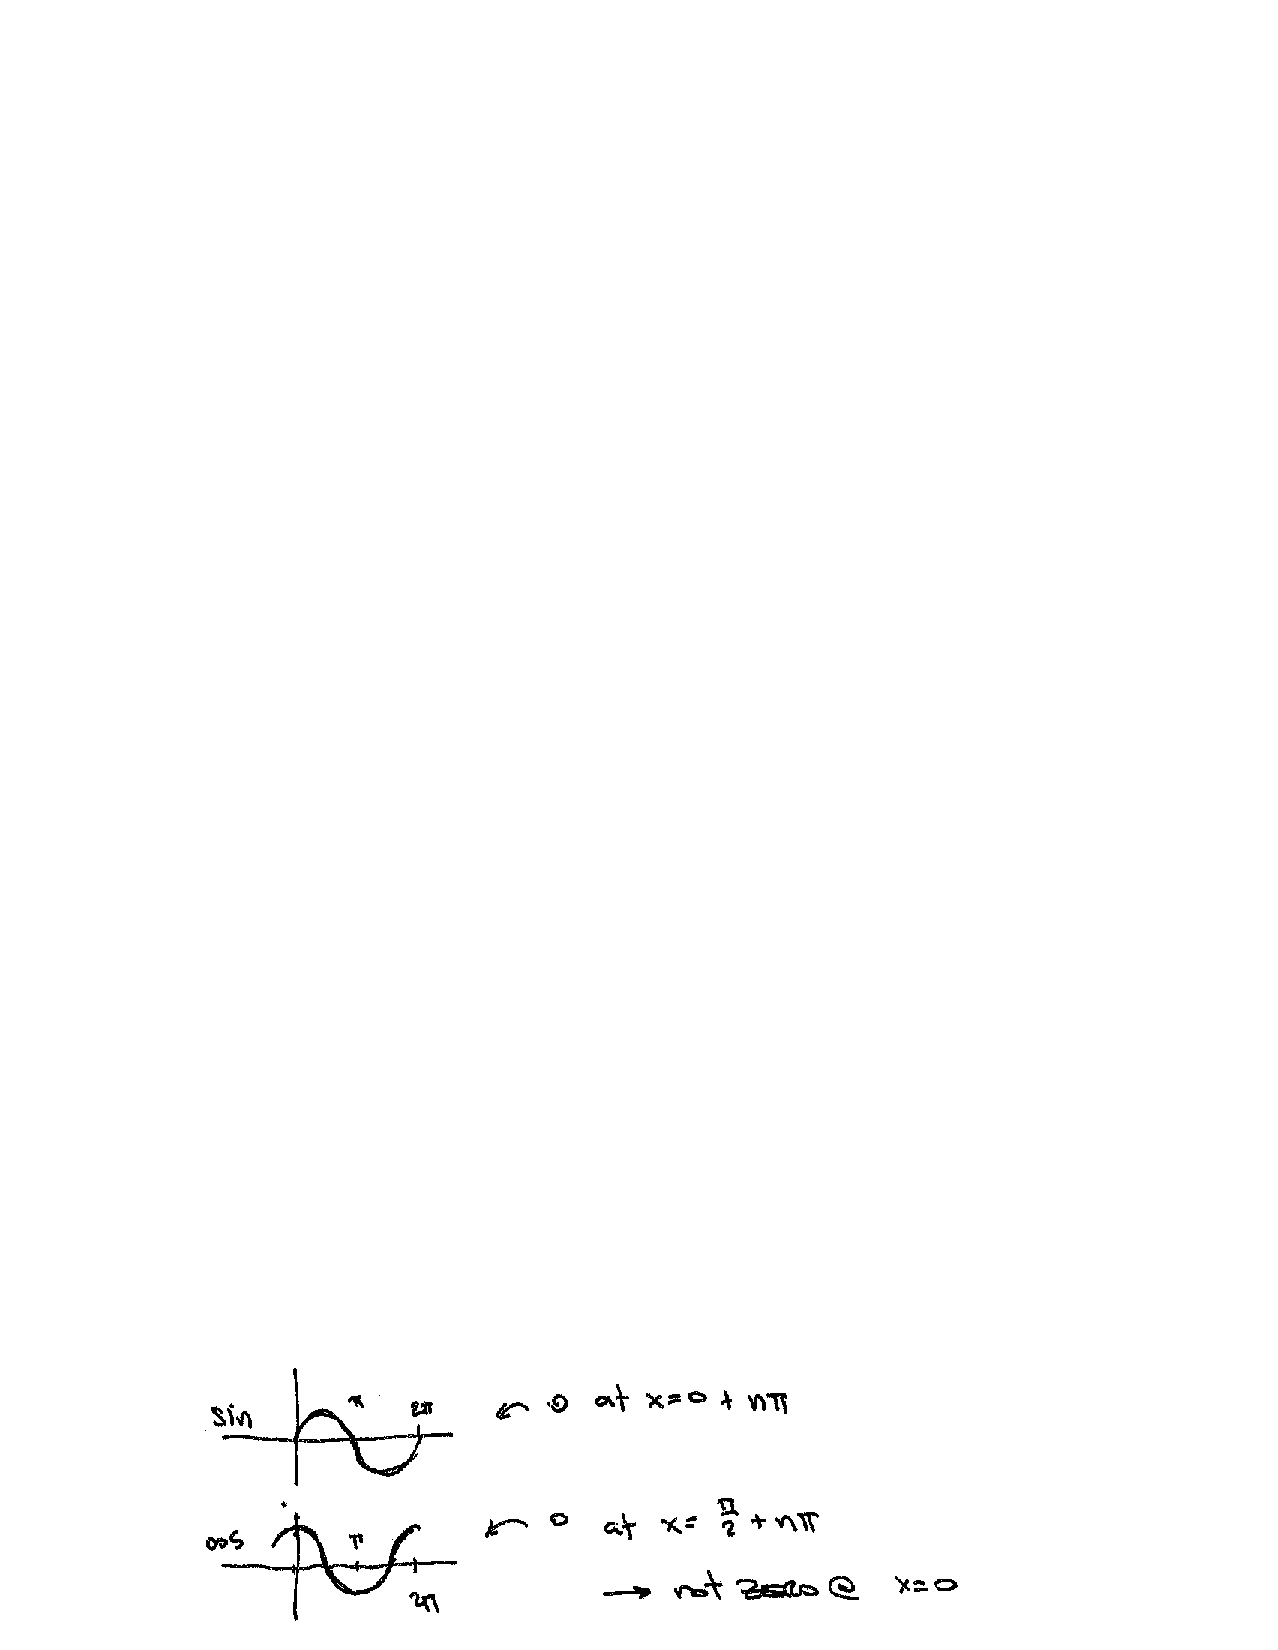
\includegraphics[width=.7\textwidth]{figures/sinesandcosines.pdf}
    \caption{Sketch of sine and cosine over one period.}
    \label{fig:sinecosine}
\end{figure}
From the plot we can see that cosine cannot satisfy the $f(0)=0$ boundary condition since this would force the coefficient to be zero. This leaves us with the sines. 

The sines automatically satisfy the $f(0)=0$ boundary condition, but do not automatically satisfy the $f(L)=0$ boundary condition. The only way for them to satisfy this boundary condition is if $x=L$ happens to coincide with one of the nodes of the sine function. The positions of the nodes are determined by the wave number, $k_n$ and occur when
\begin{align}
    k_n &= \frac{n\pi}{L} \ 
    &
    n\in \mathbbm{Z} \ .
\end{align}
We normalize these functions so that $\la f_n, f_n \ra = 1$. If we write $f_n = A_n\sin(n\pi x/L)$, means calculating
\begin{align}
    \la f_n, f_n \ra = 
    \int_0^L dx\, A_n^2 \sin^2\left(\frac{n\pi x}{L}\right)
    =
    \int_0^1 dy\, A_n^2 L \sin^2\left(n\pi y\right) \ .
\end{align}
You can plug this into your favorite calculator, or you can try to be a little clever. One approach is sketched in Fig.~\ref{fig:sinecosine:area}.
\begin{figure}[tb]
    \centering
    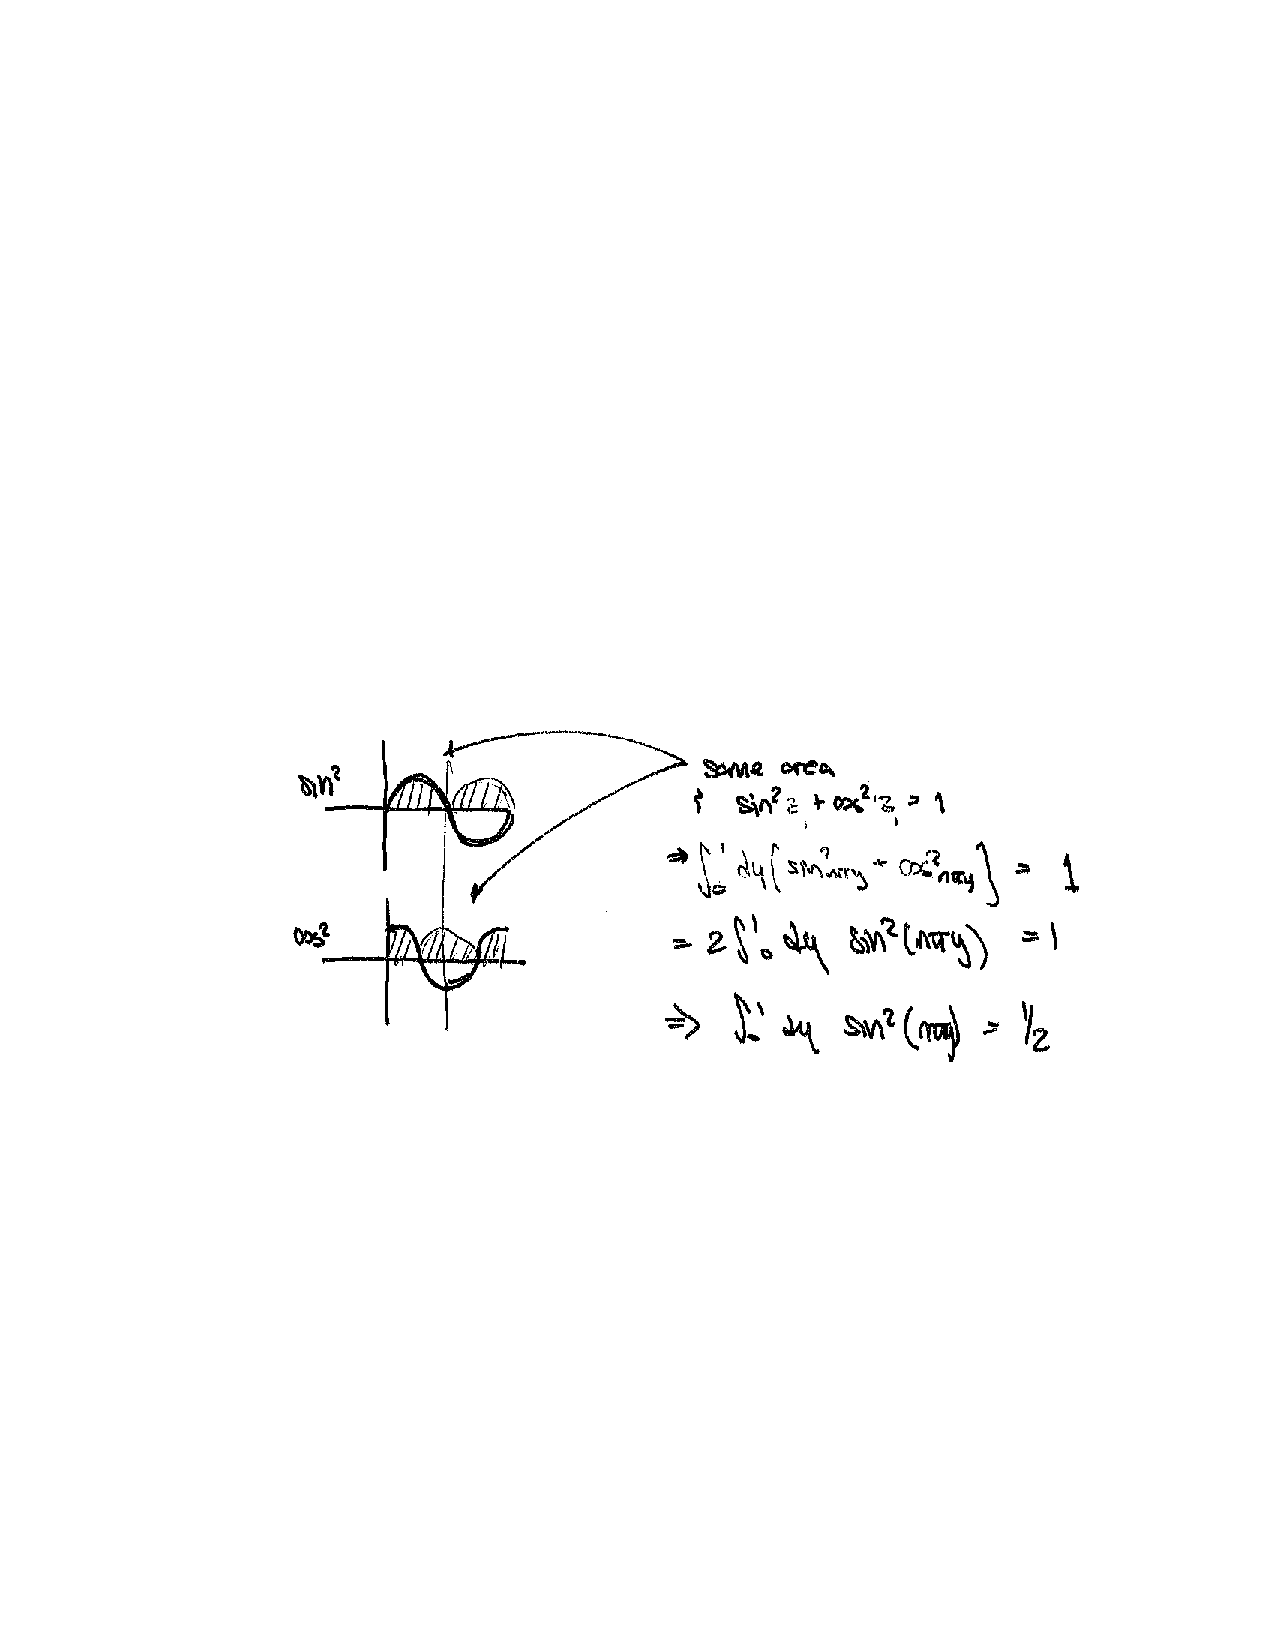
\includegraphics[width=.7\textwidth]{figures/sinecos_area.pdf}
    \caption{Sketch argument for the area under $\sin^2(k_n x)$ integrated over a period. We use $\sin^2 + \cos^2 = 1$ and the observation that both of these functions have the same area when integrated over a half-period.}
    \label{fig:sinecosine:area}
\end{figure}
This gives us an overall coefficient $\sqrt{2/L}$.

What about orthogonality? One can simply appeal to our result that the eigenfunctions of Hermitian operators like $(d/dx)^2$ are orthogonal. To check this, we need to show that
\begin{align}
    \la f_n, f_{m\neq n}\ra 
    = \int_0^L dx\, A_nA_m 
    \sin\left(\frac{n\pi x}{L}\right)
    \sin\left(\frac{m\pi x}{L}\right)
    = 0 \ .
\end{align}
One way to calculate this without appealing to a calculator is to appeal to the complex exponential representation,
\begin{align}
    \sin(n\pi y) = \frac{1}{2i}\left(e^{in\pi y} - e^{-in\pi y}\right)
\end{align}
so that the product of sines is
\begin{align}
    \sin(n\pi y)\sin(m\pi y)
    \propto 
    e^{i(m+n)\pi y} - e^{i(m-n)\pi y} - e^{i(n-m)\pi y} + e^{-i(m+n)\pi y} \ .
\end{align}
When integrating over a half-period, each term cancels pair-wise unless  $m=n$, in which case the two middle terms give non-zero contributions. 


We thus find that the eigenbasis for $(d/dx)^2$ on $x\in [0,L]$ with Dirichlet boundary conditions are the functions
\begin{align}
    f_n(x) = \sqrt{\frac{2}{L}}\sin\left(\frac{n\pi x}{L}\right) \ .
\end{align}
We see that the \emph{spectrum} of eigenvalues are \emph{quantized}. The origin of this quantization stems from the fact that the functions are defined on a finite interval. One boundary condition projected out the cosine solutions, while the other imposed a condition on the wavenumbers. The latter condition is a quantization condition because it required that the wavenumber coincide with one of the (discrete) nodes of the sine function.

\begin{exercise}
Show that Neumann and periodic boundary conditions also quantize the spectrum of eigenvalues of $(d/dx)^2$ over a finite interval.
\end{exercise}




\subsection{Example: infinite square well}

% Lesson: picks out the characteristic size of the problem
\paragraph{Quantum mechanics}
Let us apply the previous mathematical example of the Dirichlet interval into a physical example in quantum mechanics. The dynamical equation for the quantum mechanics of a non-relativistic particle with mass $m$ and time-independent potential $V(x)$ is called the Schr\"odinger equation:
\begin{align}
    i\hbar \frac{\partial \Psi(x,t)}{\partial t}
    = -\frac{\hbar}{2m}\frac{\partial^2 \Psi(x,t)}{\partial x^2} + V(x)\Psi(x,t) \ ,
\end{align}
where $\hbar$ is Planck's constant. Let us assume this equation.\footnote{For my tastes, the best ``derivation'' comes from starting from a more sophisticated relativistic theory and taking the non-relativistic limit. I advocate for not dwelling too much on the origin of the Schr\"odinger equation for our present purposes.} $\Psi(x,t)$ is the \textbf{wavefunction} of the particle. The significance is that:
\begin{enumerate}
    \item The probability that the particle is within $\varepsilon$ of $x$ at time $t$ is $\int_{x-\varepsilon}^{x+\varepsilon}dx'\, |\Psi(x',t)|^2$. This also gives a natural normalization for $\Psi$: $\int dx'\,|\Psi(x',t)|^2 = 1$ when integrated over the entire domain of $x$.
    \item Let $\mathcal O$ be a Hermitian operator corresponding to a physical observable property of the particle. The possible observable values are the eigenvalues of $\mathcal O$. If the wavefunction is a linear combination of eigenfunctions of $\mathcal O$, $\Psi(x,t) = \sum_{i}\alpha_i\Psi_{(i)}(x,t)$, then the probability of observing the eigenvalue $\lambda_i$ is $|\alpha_i|^2$. 
\end{enumerate}

\paragraph{Separation of variables} This equation simplifies if we hone in on the condition that $V(x)$ only depends on position $x$ and not time $t$. We say that the system is time independent. We have one trick that is a good starting point for partial differential equations: let us make the guess (``ansatz'' if you're mathematical) that \emph{maybe} the solution $\Psi(x,t)$ factorizes into the product of two functions of a single variable:
\begin{align}
    \Psi(x,t) = \psi(x) f(t) \ .
\end{align}
This means that the Schr\"odinger equation takes the form
\begin{align}
    \frac{i\hbar}{f}\frac{df}{dt} = -\frac{\hbar^2}{2m} \frac{1}{\psi}\frac{d^2\psi}{dx^2} + V(x) \ ,
    \label{eq:separation:of:schrodinger}
\end{align}
where we have divided through by  $\psi(x)f(t)$ to make the following point. In \eqref{eq:separation:of:schrodinger}, the left-hand side is an that is independent of $x$. On the right-hand side is an expression that is independent of $t$. Because the two are equal, both sides must be independent of both $x$ and $t$: in other words, both sides are constant. 
\begin{bigidea}
Please be sure that you thoroughly follow the slick line of thought here. 
\end{bigidea}
With the benefit of foresight, we call this constant $E$ and identify it with the energy of the system. 

\paragraph{The time equation} Equating the left-hand side of \eqref{eq:separation:of:schrodinger} to $E$ gives
\begin{align}
    i\hbar \frac{df(t)}{dt} &= E f(t)
    &
    f = A e^{-iEt/\hbar} \ .
    \label{eq:TISE:infinite:f}
\end{align}
The coefficient $A$ can be absorbed into the definition of the constant $E$. In other words, it can be absorbed into the $\psi$ equation. Observe that this tells us that the time-dependence of a stationary state is
\begin{align}
    \Psi(x,t) = e^{-iEt/\hbar} \psi(x) \ .
\end{align}
The time-dependent factor is a number of modulus 1 (part of the unit complex circle) that has a phase that advances with `speed' $E/\hbar$. 

\paragraph{Spatial equation} Equating the left-hand side of \eqref{eq:separation:of:schrodinger} to $E$ gives the time-independent Schr\"odinger equation,
\begin{align}
    \frac{-\hbar}{2m}\frac{d^2\psi(x)}{dx^2} + V(x)\psi(x) = E\psi(x) \ .
\end{align}
Observe that this takes the form of an eigenvalue equation $\mathcal O \psi = E \psi$ with operator
\begin{align}
    \mathcal O &= \frac{-\hbar}{2m}\frac{d^2}{dx^2} + V(x)
    \label{eq:time:independent:schrodinger:operator} \ .
\end{align}

\paragraph{Infinite square well potential} To make progress, let us assume a simple form for the potential in \eqref{eq:time:independent:schrodinger:operator}. 
A good example is the infinite square well, which we sketch in Ref.~\ref{fig:inf:well}:
\begin{figure}[tb]
    \centering
    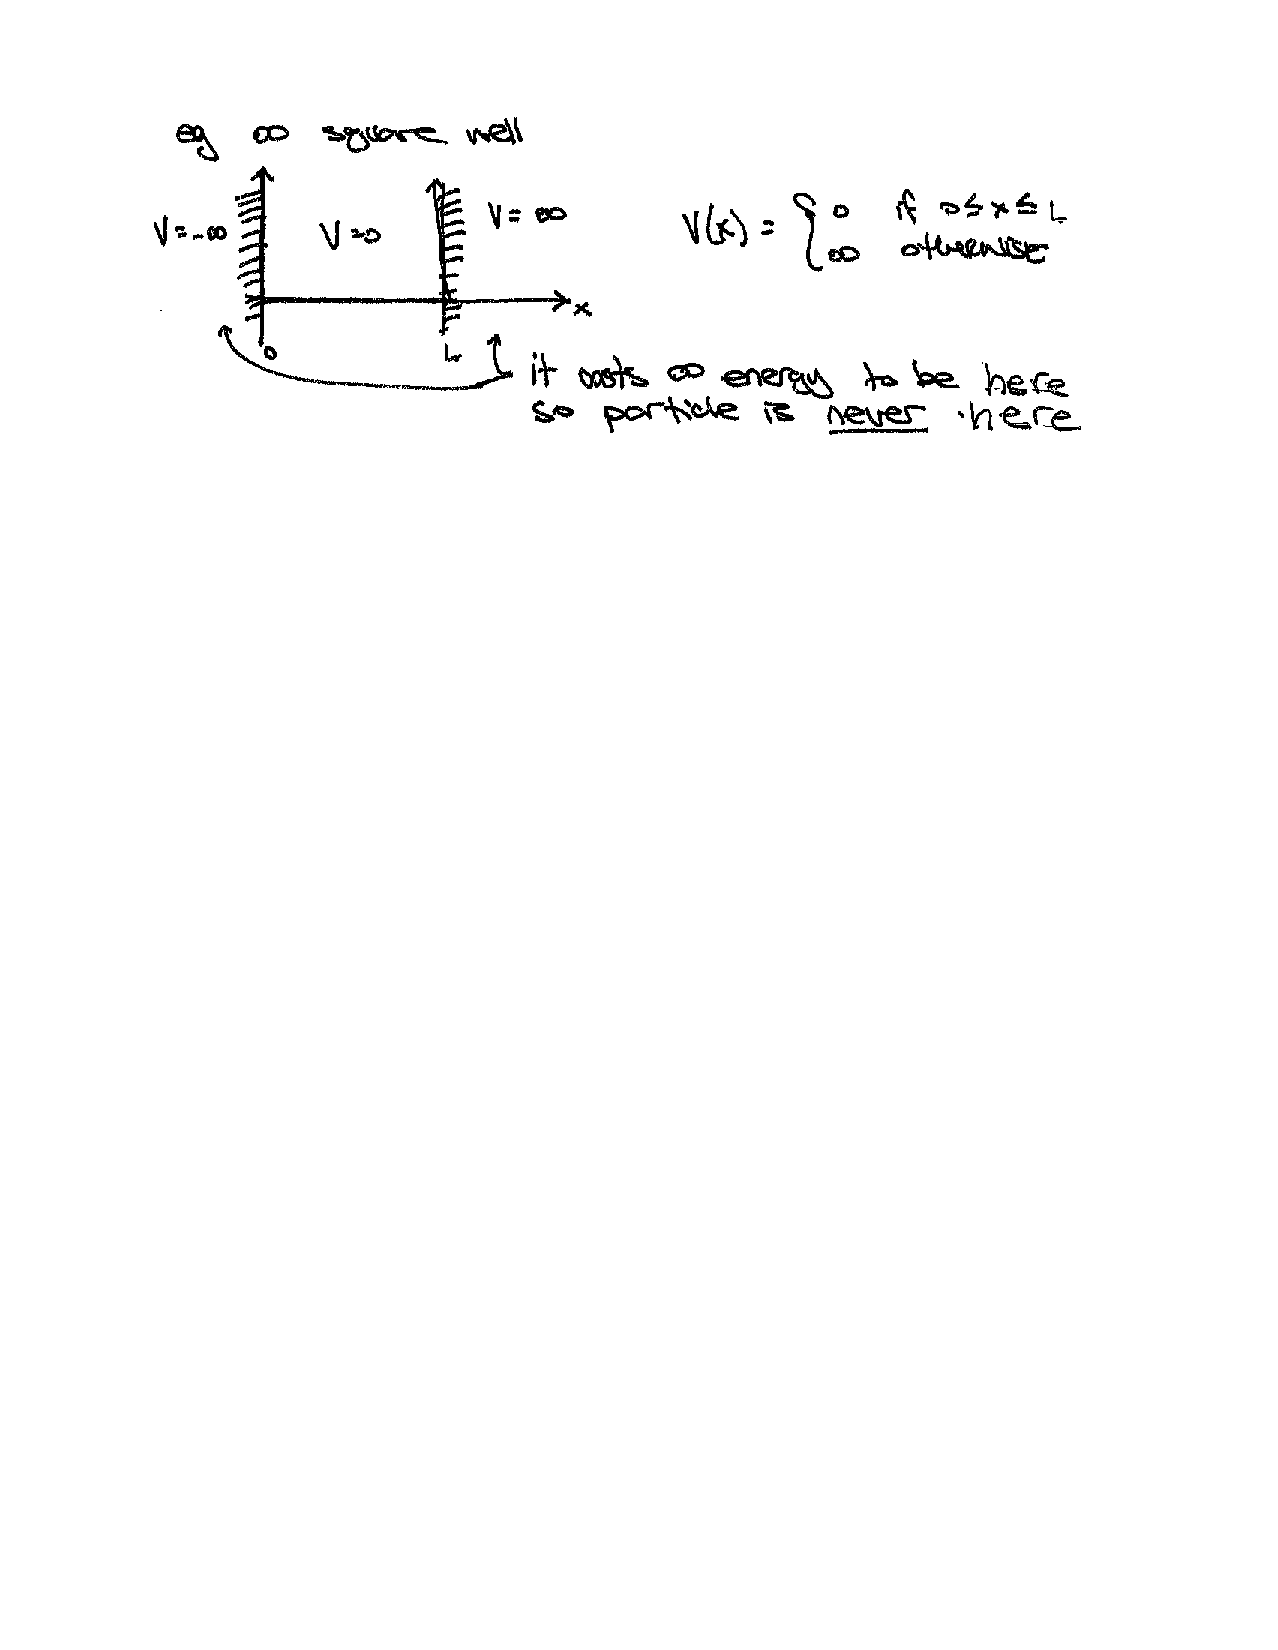
\includegraphics[width=.8\textwidth]{figures/inf_sq_well.pdf}
    \caption{The infinte square well potential equates the potential outside of $x\in[0,L]$ with $\infty$.}
    \label{fig:inf:well}
\end{figure}
The potential is essentially zero in the interval $x\in[0,L]$ and infinite outside. This means that it costs the particle an \emph{infinite} amount of energy to exist outside of the interval. That may sound pretty extreme, but quantum mechanics is weird enough that a quantum particle may ``leak out'' of any interval that does not formally have infinite barriers like this. The infinite potential essentially sets a domain for the particle $x\in[0,L]$ with Dirichlet boundary conditions. 
\begin{exercise}
In your own words, justify why the infinite square well requires Dirichlet boundary conditions at $x=0$ and $x=L$.
\end{exercise}

If we rearrange a few terms, we end up with a time-independent Schr\"odinger equation for the infinite square well:
\begin{align}
    \left(\frac{d}{dx}\right)^2 \psi(x) = -\frac{2mE}{\hbar^2}\psi(x) 
    = - k^2 \psi(x) \ .
    \ ,
    \label{eq:TISE:infinite:well:2nd:O}
\end{align}
where we understand that the full wavefunction $\Psi(x,t)$ is $\psi(x)$ multiplied by the phase factor \eqref{eq:TISE:infinite:f}. We now see that our equation is the $(d/dx)^2$ eigenvalue equation for the Dirichlet interval with eigenvalue $-k^2 = -2mE/\hbar^2$. We know all about the solutions to this equation from the previous subsection:
\begin{align}
    \psi(x) &= \sqrt{\frac{2}{L}} \sin(k_n x)
    &
    k_n &= \frac{n\pi}{L} \ .
\end{align}
We have a spectrum of wave numbers, $k_n$. Equating the wave numbers to $k$ in \eqref{eq:TISE:infinite:well:2nd:O} gives a discrete spectrum of energies:
\begin{align}
    E_n = \frac{n^2 \pi^2 \hbar}{2mL^2} \ .
\end{align}
While we have not formally justified why the constant $E$ is an energy, we \emph{have} shown that the separation of variables trick can only work if $E$ inherits the discrete spectrum of wave numbers. 

\begin{example} What is the wavefunction of a particle in an infinite square well of length $L$ and energy $E_2 =  2^2 \pi^2 \hbar / 2mL^2$? We find
\begin{align}
    \psi(x) = \frac{2}{L} \sin\left(\frac{2\pi x}{L}\right) \ .
\end{align}

\end{example}



\begin{subappendices}
\section{\texorpdfstring{The $\delta$ function}{The Delta Function}}

The Dirac $\delta$ function\sidenote{The $\delta$ function is not formally a function. It is an object called a \emph{distribution} that only makes sense when integrated over.} is defined to be the distribution over which
\begin{align}
    \int_{-\infty}^\infty \D{x}\, f(x)\delta(x-y) &= f(y) \, .
\end{align}
In fact, we may more carefully refine this:
\begin{align}
\lim_{\epsilon \to 0}
    \int_{y-\epsilon}^{y+\epsilon} \D{x}\, f(x)\delta(x-y) &= f(y) \, .
\end{align}
In this definition, it is clear that the entirety of the support\sidenote{Support means the region where something is nonzero} of $\delta(x-y)$ is an infinitesimal sliver around $x=y$. One can compare this to the Kronecker $\delta$ in a sum:
\begin{align}
    \sum_i \Delta x\; \delta^j_i v^i = v^j \ ,
\end{align}
where we have explicitly written in $\Delta x = 1$. If you want to make the comparison closer, you could imagine writing a two-argument function $\delta(x,y)\defeq \delta(x-y)$ and treat the $x$ and $y$ as continuous `indices.'

We make a key observation that the $\delta$ function has infinitesimal support. It is zero \emph{everywhere} except for a set of measure zero.\sidenote{This is a mathy way of saying: you may be looking at the real line, but the the function is only non-zero at a single point. This point has no `length' or spatial extent.} However, it integrates to one, so it has unit area under its odd curve.

We may motivate the $\delta$ function in a limiting procedure. Some textbooks like to do this by writing out a function that becomes skinnier and taller in some limit. That is a little dishonest because the $\delta$ function is really the degenerate extreme of that limit. Instead, let us consider the limiting procedure of the $\delta$ function integrated over some test function, $f(x)$. First let us imagine a pre-$\delta$ function that we call $\tilde \delta(x)$. As a first iteration, we sketch it in Figure~\ref{fig:delta:limit:1}.

\begin{marginfigure}%[th]
    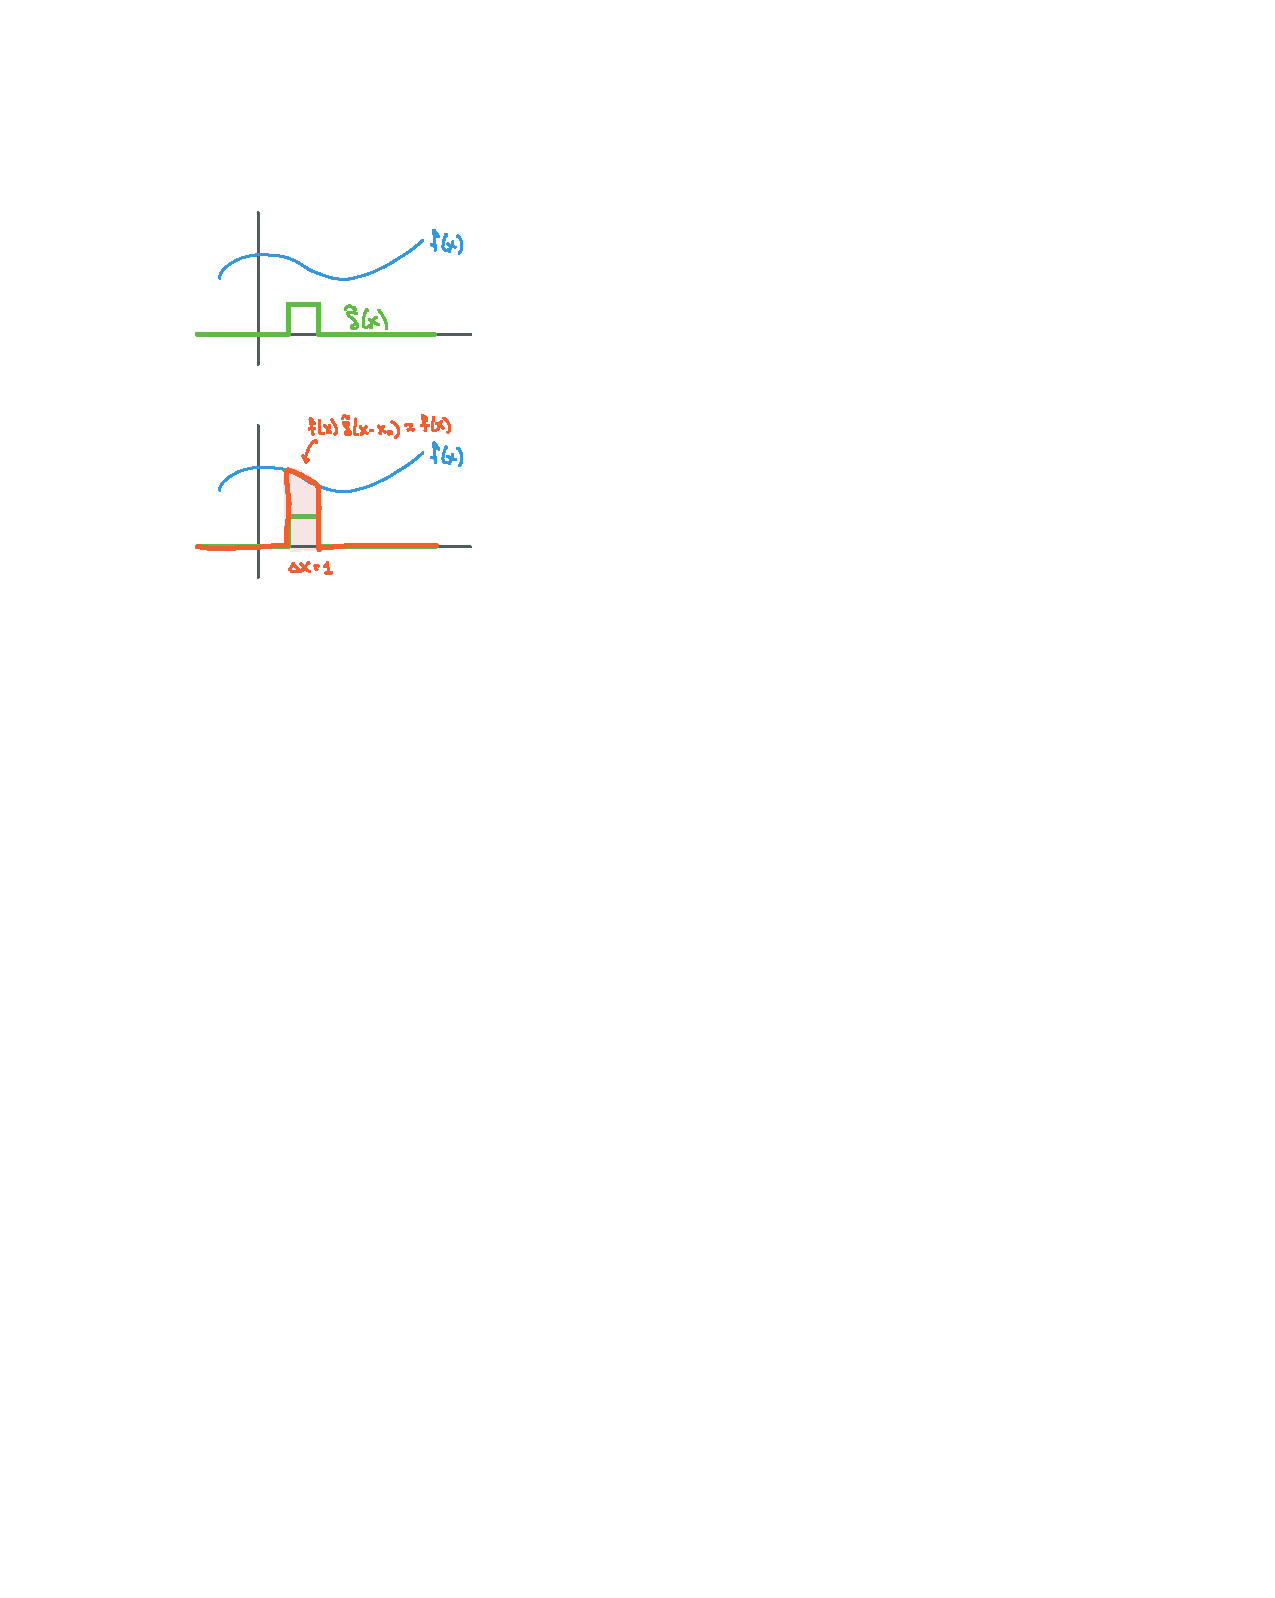
\includegraphics[width=\textwidth]{figures/Delta_limit_01.pdf}
    \captionsetup{font={scriptsize,sf}}
    \caption{A pre-$\delta$ function, $\tilde \delta(x)$, green. In the lower plot, we show the area under the curve $f(x)\tilde\delta(x-x_0)$. Observe that $f(x)\tilde\delta(x-x_0)$ is zero everywhere except in the region of size $\Delta x=1$ around $x_0$. For $\Delta x =1$, the non-zero region traces $f(x)$. }
    \label{fig:delta:limit:1}
\end{marginfigure}

In this picture, we assume that $\tilde\delta(x-x_0)$ is zero everywhere except for a region of width $\Delta x = 1$ around $x_0$. In that region, we write that $\tilde\delta(x-x_0)$ has height $\Delta x\inv = 1$. This means that the product with a test function $f(x)$ satisfies
\begin{align}
    f(x)\tilde\delta(x-x_0)
    =
    \begin{cases}
    \frac{f(x)}{\Delta x} &\text{if } x_0-\frac{\Delta x}{2} \leq x \leq x_0 +\frac{\Delta x}{2} \\
    0 &\text{otherwise}
    \end{cases}
    \ ,
\end{align}
where $\Delta x = 1$ in Figure~\ref{fig:delta:limit:1}. This means that the area under $f(x)\tilde\delta(x-x_0)$ is the area under $f(x)$ in the unit region around $x_0$. 

We can now imagine making $\Delta x$ successively smaller, for example in Figure~\ref{fig:delta:limit:2} we take $\Delta x = 1/2$. Observe that because $\Delta x$ is smaller, the value of $f(x)\tilde\delta(x-x_0)$ is larger---at least in the [smaller] region where $\tilde\delta(x-x_0)$ is non-zero. 
\begin{marginfigure}%[th]
    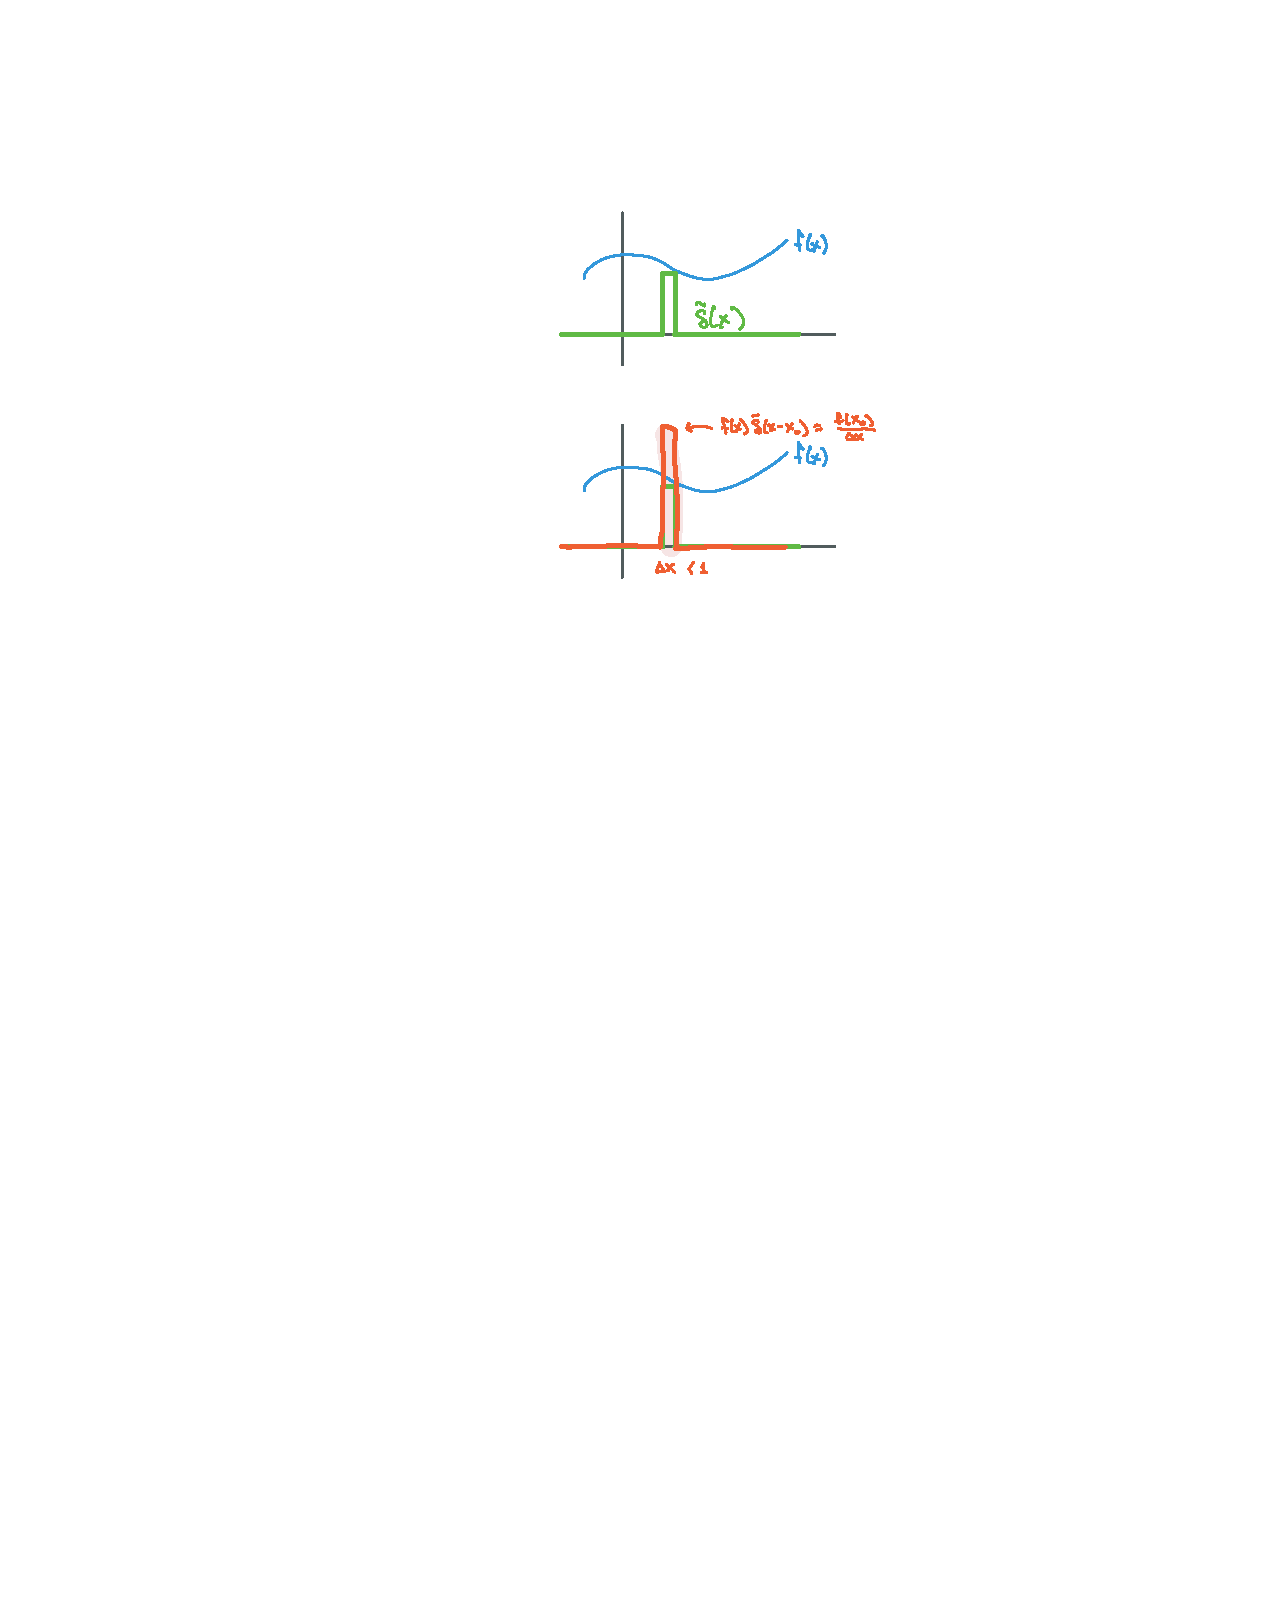
\includegraphics[width=\textwidth]{figures/Delta_limit_02.pdf}
    \captionsetup{font={scriptsize,sf}}
    \caption{Same as above, but with $\Delta x = 1/2$. The product $f(x)\tilde \delta(x-x0)$ is now $f(x)/\Delta x$ in the sliver of extent $\Delta x$ around $x_0$ where it is nonzero.}
    \label{fig:delta:limit:2}
\end{marginfigure}
As we take the limiting case where $\Delta x$ is smaller than any characteristic scale over which $f(x)$ changes appreciably, we find that the integral over $f(x)\tilde\delta(x-x_0)$ is approximately
\begin{align}
    \int_{-\infty}^\infty \D{x}\, f(x)\tilde\delta(x-x_0) = \frac{f(x_0)}{\Delta x} \Delta x = f(x_0) \ .
\end{align}
This becomes exact as $\Delta x \to 0$ and the $\tilde\delta(x)\to \delta(x)$ function becomes infinitely tall and infinitesimally thin but maintains unit area under its curve.

The $\delta$ function cancels an integral in the same way that a Kronecker $\delta$ cancels a sum: It replaces the integral with the integrand evaluated at a single point:

While $\delta$ functions may look like a silly way of writing a function, they serve as basis dual functions in function space written in the position basis. In physics they are clever ways to write out constraints. For example, the unit circle is a one dimensional slice of the two-dimensional plane. One way of writing this integral is to integrate some function $f(x,y)$ along the plane but restrict the integral to the unit circle in the following way:
\begin{align}
    \int \D{x}\D{y}\; \delta(x^2 + y^2 - 1) \, f(x,y) \ .
\end{align}

The example above brings us to the question of how to evaluate a $\delta$ function when the argument is not linear in the integration variable. That is, what do you do with $\D{x}\, \delta(f(x))$? The trick here is to do a change of variables where $u = f(x)$.
\begin{align}
    \int \D{x}\, \delta(f(x))\, g(x)
    &= 
    \int \frac{\D{u}}{|f'(x(u))|} \, \delta(u) \, g(x(u))
    \\
    &= \sum_i\frac{g(x_i)}{|f'(x_i)|} \ ,
\end{align}
where the points $x_i$ are the points for which $f(x_i) = 0$. This gives us a rule that
\begin{align}
    \delta(f(x)) &= \sum_i \frac{\delta(x-x_i)}{f'(x_i)} \ .
\end{align}

\paragraph{That's not how I learned it...} Many standard undergraduate mathematical physics textbooks present the Dirac $\delta$ function as the limiting form of ordinary functions. The representation as an infinitely skinny Gaussian normalized to unit area is a popular one. When treated carefully, these limits give meaningful results and are a suitable working definition for the Dirac $\delta$ function. However, one danger of that picture is that the reader may be led to believe that $\delta$ functions are... functions. From the perspective developed in this course, $\delta$ functions are \emph{not} functions. They are \emph{distributions} that \emph{only} make sense when integrated over. 

Consider a probability distribution, $p(x)\,\D{x}$ defined over $x\in [a,b]$. This satisfies $\int_a^b \D{x}\, p(x) = 1$ and has an interpretation that
$
    \int_c^d \D{x}\, p(x)
$
is the probability that $x \in [c,d]$, where we assume $a\leq c < d \leq b$. The mathematical expression for $p(x)$ may be perfectly well behaved; perhaps it looks something like a Gaussian. However, as a \emph{distribution} you should \emph{never} separate $p(x)$ from $\D{x}$: the distribution is $p(x)\,\D{x}$ and it only makes sense when you are integrating it over another function. The Dirac $\delta$ is the limit where $x$ has some definite value. Formally, we should only write $\delta(x-x_0)\,\D{x}$.

In this way, distributions are not functions, but \emph{dual functions} in the way that row vectors are dual vectors. Distributions are the linear functions on the space of functions. You give a distribution a function, and it spits out a number that is defined by the integral of that function over the distribution. 
\begin{align}
    \la \delta(x-x_0) \mid f \ra = \int \D{x}\, \delta(x-x_0)\, f(x) = f(x_0) \ .
\end{align}






\end{subappendices}

